%!TEX options = -shell-escape

\documentclass[a4paper]{article}

% Suppress some useless warnings
\usepackage{silence}
\WarningFilter{remreset}{The remreset package}
\WarningFilter{latex}{Font shape declaration has incorrect series value `mc'.}

\usepackage[UKenglish]{babel}
\usepackage[style=alphabetic,maxbibnames=99]{biblatex}
\usepackage{amsmath}
\usepackage{mathtools}
\usepackage{amsthm}
\usepackage{thmtools}
\usepackage{csquotes}
\usepackage{commath}
\usepackage{url}
\usepackage{algorithm}
\usepackage{algpseudocode}
\usepackage[inline]{enumitem}
\usepackage[hidelinks]{hyperref}
\usepackage[capitalize,noabbrev]{cleveref}
\usepackage[final]{microtype}
\usepackage{caption}
\usepackage{subcaption}

\usepackage[charter]{mathdesign}
\usepackage[T1]{fontenc}

% Fix me notes
\usepackage[draft]{fixme}
\usepackage{svg}
\fxusetheme{color}

% Theorem styles
\newtheorem{theorem}{Theorem}
\newtheorem{lemma}[theorem]{Lemma}
\newtheorem{proposition}[theorem]{Proposition}
\newtheorem{corollary}[theorem]{Corollary}
\newtheorem{question}[theorem]{Question}
\newtheorem*{mainquestion}{Main question}
\theoremstyle{definition}
\newtheorem{definition}[theorem]{Definition}
\newtheorem{construction}[theorem]{Construction}
\newtheorem{example}[theorem]{Example}
\theoremstyle{remark}
\newtheorem{remark}[theorem]{Remark}

% LaTeX shorthands
% Single letters
\newcommand{\R}{\ensuremath{\mathbb{R}}}
\newcommand{\Q}{\ensuremath{\mathbb{Q}}}
\newcommand{\Z}{\ensuremath{\mathbb{Z}}}
\newcommand{\N}{\ensuremath{\mathbb{N}}}
\newcommand{\D}{\ensuremath{\mathcal{D}}}

% Shorthands
\newcommand{\ep}{\epsilon}
\newcommand{\lam}{\lambda}
\newcommand{\Lam}{\Lambda}
\newcommand{\la}{\leftarrow}
\newcommand{\ra}{\rightarrow}
\newcommand{\lra}{\leftrightarrow}
\newcommand{\La}{\Leftarrow}
\newcommand{\Ra}{\Rightarrow}
\newcommand{\Lra}{\Leftrightarrow}
\newcommand{\es}{\varnothing}
\newcommand{\sse}{\subseteq}
\newcommand{\partto}{\rightharpoonup}
\newcommand{\ol}{\overline}
\newcommand{\wt}{\widetilde}
\newcommand{\wh}{\widehat}
\newcommand{\bb}{\mathbb}
\newcommand{\mc}{\mathcal}
\newcommand{\mr}{\mathrm}
\newcommand{\defeq}{\vcentcolon=}
\DeclarePairedDelimiter{\ab}{\langle}{\rangle}
\let\abs\undefined
\DeclarePairedDelimiter{\abs}{|}{|}

% Slanted symbols
\renewcommand{\leq}{\leqslant}
\renewcommand{\geq}{\geqslant}
\renewcommand{\nleq}{\nleqslant}
\renewcommand{\ngeq}{\ngeqslant}

% Bibliography
\addbibresource{../references.bib}

\title{Reproducing the paper:\\
\textit{Stochastic Gradient Hamiltonian Monte Carlo}\\
by Tianqi Chen, Emily B. Fox and Carlos Guestrin}
\author{Sam Adam-Day, Alexander Goodall, Theo Lewy and Fanqi Xu}
\date{}

\begin{document}

	\maketitle

	\abstract{We reproduce the experiments contained in \citetitle{sghmc} \cite{sghmc} by \citeauthor{sghmc}.\fxnote{Give more details in abstract}}

	\listoffixmes

	%!TEX root = ../report.tex

\section{Introduction}

Hamiltonian Monte Carlo (HMC) methods already provide a way to sample from a posterior distribution. These methods use all data available to them to produce a potential energy function $$U(\theta) = - \sum_{x\in\mathcal{D}}\text{log}(p(x| \theta)) - \text{log}(p(\theta )) \propto -\text{log}(p(\theta | \mathcal{D}))$$
which, along with $\nabla U(\theta)$, is sufficient to sample from the posterior (as will be discussed in the background section). Computing $U(\theta)$ and $\nabla U(\theta)$ can be computationally expensive for large datasets, and so research into Stochastic Gradient Hamiltonian Monte Carlo (SGHMC) methods began (\cite{sghmc}), which use subsets of the data to produce noisy estimates of $U(\theta)$ and $\nabla U(\theta)$. We decided to investigate this paper. It starts with a description of HMC, and then introduces a Naive SGHMC algorithm. It then goes on to introduce SGHMC (the main algorithm), and then it runs a number of experiments using these algorithms.

Our motivation to choose this paper stemmed from the fact that the SGHMC algorithm is relatively simple, and so we would have more time to investigate other datasets and ideas. It is also computationally fast, allowing us to run experiments on our home computers. We reproduced the following experiments from \cite{sghmc}:

\begin{itemize}
    \item Sampling $\theta$ from the posterior with $U(\theta) = -2\theta^2 + \theta^4$ using HMC, Naive SGHMC and SGHMC
    \item Sampling $(\theta,r)$ generated from $U(\theta) = \frac{1}{2}\theta^2$ with HMC, and from $U(\theta) = \frac{1}{2}\theta^2 + \mathcal{N}(0,4)$ as a proxy for SGHMC
    \item Classifying the MNIST dataset using SGHMC as well as with Stochastic Gradient Descent, Stochastic Gradient Descent with momentum, and Stochastic Gradient Langevin Dynamics
\end{itemize}

We also considered some new ideas:

\begin{itemize}
    \item We extended the 'No U-Turn Sampler' (NUTS) from \cite{nuts} to work with SGHMC to produce our novel algorithm SGNUTS
    \item We ran experiments on a new dataset of FashionMNIST
    \item We briefly introduced some Convolutional Neural Networks (CNNs) to see how accurate SGHMC was at classifying CIFAR10
    \item We attempted to evaluate the noisiness of the data ($B$ in the literature and in what follows) and used this to increase the algorithm's efficiency
\end{itemize}

The repository for our code is found at https://github.com/sacktock/SGHMC.

	%!TEX root = ../report.tex

\section{Background}

\subsection{HMC}

Hamiltonian Monte Carlo (\cite{duane-hmc,neal-hmc}) is a Markov Chain Monte Carlo (MCMC) sampling algorithm. Given a target probability distribution — in our case the posterior distribution of a set of variables $\theta$ given independent observations $x \in \D$ — it produces samples by carrying out a random walk over the parameter space using Hamiltonian dynamics.

We begin with the prior distribution $p(\theta)$ and likelihood $p(x \mid \theta)$. Using these we define the \emph{potential energy} function $U$:
\begin{equation*}
    U(\theta) \defeq - \sum_{x \in \D}\log p(x \mid \theta) - \log p(\theta)
\end{equation*}
Note that, using Bayes' rule, we have that the posterior $p(\theta \mid \D) \propto \exp(-U)$. Hamiltonian dynamics introduces an auxiliary set of momentum variables $r$. These dynamics have a physical interpretation in which an object moves about a landscape determined by $U$. We let this object have \emph{mass matrix} $M$, which is typically set to the identity matrix. Then $U(\theta)$ represents the potential energy of the object, and its kinetic energy is given by $\frac 1 2 r^{\mathsf T} M^{-1} r$. The total energy of the system is a quantity known as the \emph{Hamiltonian function}:
\begin{equation*}
    H(\theta, r) = U(\theta) + \frac 1 2 r^{\mathsf T} M^{-1} r
\end{equation*}
The development of the system is governed by the following equations.
\begin{align*}
    \dif\theta &= M^{-1}r \dif t \\
    \dif r &= - \nabla U(\theta) \dif t
\end{align*}

To simulate these continuous dynamics in practice, we must use a discretised version of these equations. To correct for the inaccuracies introduced by doing so, it is necessary to make a \emph{Metropolis-Hastings correction step}. A simple algorithm is given in \cref{alg:hmc}.

\begin{algorithm}
    \caption{A simple HMC algorithm}\label{alg:hmc}
    \begin{algorithmic}
        \For{$t = 1,2, \ldots$}
            \State $r \sim \mc N(0,1)$ \Comment{Resample momentum}
            \State $(\theta_0, r_0) = (\theta, r)$ 
            \For{$i = 1$ to $m$}
                \State $\theta \gets \theta + \ep M^{-1}r$
                \State $r \gets r - \ep \nabla U(\theta)$
            \EndFor
            \State $u \sim \rm{Uniform}[0,1]$
            \State $\rho = \exp(H(\theta, r) - H(\theta_0, r_0))$ \Comment{Acceptance probability}
            \If{$u < \min(1, \rho)$} \Comment{Only accept new state with probability $\rho$}
                \State $\theta = \theta_0$
            \EndIf
        \EndFor
    \end{algorithmic}
\end{algorithm}

In practice, the dataset $\D$ may be large, and so running \cref{alg:hmc} may be computationally expensive, as the complexity of calculating $\nabla U$ scales with $\abs\D$. One idea to combat this is to simulate the Hamiltonian system using only a subset of the data at a time, in analogy with stochastic gradient descent. This method is known as Stochastic Gradient Hamiltonian Monte Carlo (SGHMC), however before explaining the SGHMC algorithm we begin with Naïve SGHMC.


\subsection{Naïve SGHMC}

To understand the Naïve SGHMC method, consider sampling a minibatch $\wt\D \subset \D$ uniformly at random. We estimate the gradient $\nabla U(\theta)$ using this minibatch as follows:
\begin{equation*}
    \nabla \wt U(\theta) = - \frac{\abs\D}{\abs{\wt\D}}\sum_{x \in \wt\D} \nabla \log p(x \mid \theta) - \nabla \log p(\theta)
\end{equation*}
Appealing to the Central Limit Theorem, we imagine that the noisy estimate $\nabla \wt U(\theta)$ is normally distributed about $\nabla U(\theta)$, with some covariance matrix $V(\theta)$. The naïve adaptation of HMC to this stochastic scenario simply replaces $\nabla U(\theta)$ with $\nabla \wt U(\theta)$ in \cref{alg:hmc}. The corresponding discrete system is then the $\ep$-discretisation of the following dynamics:
\begin{align*}
    \dif\theta &= M^{-1}r \dif t \\
    \dif r &= - \nabla U(\theta) \dif t + \mc N(0, 2B(\theta) \dif t)
\end{align*}
where $B(\theta) = \frac 1 2 \ep V(\theta)$.

Unfortunately, such a dynamical system can diverge quite rapidly from the true posterior distribution \cite{neal-hmc}, which necessitates frequent Metropolis-Hastings steps. Such steps are costly since calculating the acceptance probability requires the use of the whole dataset. The method `Stochastic Gradient Hamiltonian Monte Carlo' (SGHMC) proposed in \cite{sghmc} addresses this shortcoming. The idea is to incorporate friction into the dynamical system, which works to counteract the noise introduced by selecting a subset of the data.


\subsection{SGHMC}

The SGHMC method adds a `friction term' $B M^{-1} r$ to the momentum update. Since we are unlikely to know the noise model $B$ in practice, we instead take an estimate $\wh B$ of $B$, together with a user-specified friction term $C \succeq \wh B$ and simulate the following dynamics.
\begin{align*}
    \dif\theta &= M^{-1}r \dif t \\
    \dif r &= - \nabla U(\theta) \dif t - CM^{-1}r \dif t + \mc N(0, 2(C - \wh B(\theta))\dif t) + \mc N(0, 2B(\theta) \dif t)
\end{align*}
The algorithm is given in \cref{alg:sghmc}. In the case where $\wh B = B$, these dynamics accurately traverse from the posterior distribution. In practice, we must rely on an inaccurate estimate $\wh B$. The simplest choice is $\wh B = 0$. A better but more costly estimate is $\wh B(\theta) = \frac 1 2 \ep \wh V(\theta)$, where $\wh V$ is the observed (empirical Fisher) information \cite{sgld-fisher}. The friction term $C$ can then be taken as a hyperparameter, and set so as to counteract the inaccuracies of the estimate $\wh B$.

\begin{algorithm}
    \caption{The SGHMC algorithm}\label{alg:sghmc}
    \begin{algorithmic}
        \For{$t = 1,2, \ldots$}
            \State $r \sim \mc N(0,1)$ \Comment{Resample momentum}
            \For{$i = 1$ to $m$}
                \State $\theta \gets \theta + \ep M^{-1}r$
                \State $r \gets r - \ep \nabla \wt U(\theta) - \ep CM^{-1}r + \mc N(0, 2(C- \wh B(\theta))\ep)$
            \EndFor
        \EndFor
    \end{algorithmic}
\end{algorithm}
	
%!TEX root = ../report.tex

\section{Implementation Details}

We implemented the following algorithms from scratch: HMC, SGHMC, SGLD (stochastic gradient Langevin dynamics \cite{sgld}), SGD (stochastic gradient descent), SGD with Nesterov momentum and SGNUTS — a novel extension to SGHMC that uses ideas from the popular No U-Turn Sampler \cite{nuts}. All of our implementations subclass Pyro's \texttt{MCMCKernel} and are designed to be used directly with Pyro \cite{pyro} — a universal probabilistic programming language (PPL) written in Python. In Pyro the user specifies a model which is a probabilistic program (PP) that describes a posterior distribution $p(\theta \: | \: \D)$ that we want to sample from; $\theta$ corresponds to the sampled parameters or latent parameters of the model and $\D$ corresponds to the observed parameters of the model. 

Pyro already comes with the following MCMC samplers: HMC, MH and NUTS. So while the algorithms we implemented are not novel they are in fact innovative since Pyro doesn't come with any of them already built. The main reason for choosing to implement our algorithms on top of Pyro is because Pyro comes with a method \texttt{initialize\_model} that given a Pyro PP or model $P$ transforms it into a potential function $U$. Once we have $U$ we can pass the latent and observed parameters $(\theta, \D)$ to $U$, which computes the negative log joint $- \log p(\theta, \D)$. Bayes' rule tells us that  $p(\theta \: | \: \D) \propto p(\theta, \D)$ which is typically all we need for MCMC samplers and even simpler ones such as Importance and Rejection samplers \cite{bishop2006pattern}. Pyro also comes with the method \texttt{potential\_grad}, which given $(\theta, \D)$ computes the gradient of $U$ with respect to the parameters $\theta$. The result is that we can specify any arbitrary PP and apply our algorithms to them — letting Pyro handle the transformation from PP to potential function and the gradient computations.

In traditional MCMC samplers the observed dataset $\D$ is constant and so once a Pyro PP has been transformed into a potential function $U(\theta) = - \log p(\theta, \D)$ we need not change it. Unfortunately this is less straight forward for stochastic gradient samplers such as SGHMC and SGLD since we subsample the full dataset $\D$ by sampling minibatches $\wt{\D}$, where $\wt{\D} \subset \D$. In both SGHMC and SGLD we require that the potential function has the form:
$$\wt{U}(\theta) =  -\frac{|\D|}{|\wt{\D}|} \log p(\wt{\D} \: | \: \theta) - \log p (\theta)$$
Unfortunately when we subsample the dataset and call \texttt{initialize\_model} Pyro doesn't explicitly supply us with the likelihood term $p(\wt{\D} \: | \: \theta)$ - it only gives us the negative log joint $- \log p(\theta, \wt{\D})$, so to get the desired behaviour above we had to get our hands dirty and modify Pyro's source code. As a result every time we generate a new sample using SGHMC or SGLD we have to call \texttt{initialize\_model} so that it gives us the correct $\wt{U}(\theta)$ for some given minibatch $\wt{\D}$, although this is a small price to pay for much quicker gradient computations.

For the estimate of $\wh B$, in our implementation we provide two options: take $\wh B = 0$ or use $\wh B(\theta) = \frac 1 2 \ep \wh V(\theta)$, where $\wh V$ is the observed information, as suggested in \cite{sghmc}. While the latter provides a better estimate, it is much slower, and requires more memory. When $\wh B$ is estimated using the observed information, we provided the option to compute it once at setup time, recalculate every sample, or recalculate every step when simulating the dynamics.
	%!TEX root = ../report.tex

\section{Experiments}

\subsection{Simulated examples}

In this next section we present the results and intuition behind the first three experiments in \cite{sghmc}. We reproduced these three experiments by converting the MATLAB codes provided by the authors \citeauthor{sghmc} \cite{simu_code} into Python code. We used this, rather than our own implementation of SGHMC, as our version does not directly interface with a given potential function, but only Pyro PPs. The experiments that we replicated consisted of checking whether the samples produced by SGHMC and the other algorithms actually follow the target distribution.

\subsubsection*{Experiment 1}

As in \cite{sghmc} we considered the potential function $U(\theta) = -2\theta^2 + \theta^4$. This is sufficient for the purpose of checking the convergence to the target distribution for HMC. To check that the theoretical convergence of Naïve SGHMC and SGHMC are true or not we first introduce noise into the gradientl, and so we set:
$$\nabla \widetilde{U}(\theta) = \nabla U(\theta) + \mathcal{N}(0,4)$$
when we consider the noisy methods. This corresponds to setting the noise covariance to $V=4$ in the description of Naïve SGHMC we gave earlier. We then take samples using HMC, Naïve SGHMC and SGHMC. We also note that both HMC and Naïve SGHMC use Metropolis Hastings corrections (MH), while SGHMC has no need to. This allows us to test 5 algorithms: HMC (with MH), HMC (without MH), Naïve SGHMC (with MH), Naïve SGHMC (without MH), and SGHMC. We not only performed the experiments on $U(\theta) = -2\theta^2 + \theta^4$, but also on $U(\theta) = \theta^2$. The results are shown in \cref{fig:demo1,fig:demo2}.

\begin{figure}[h!]
  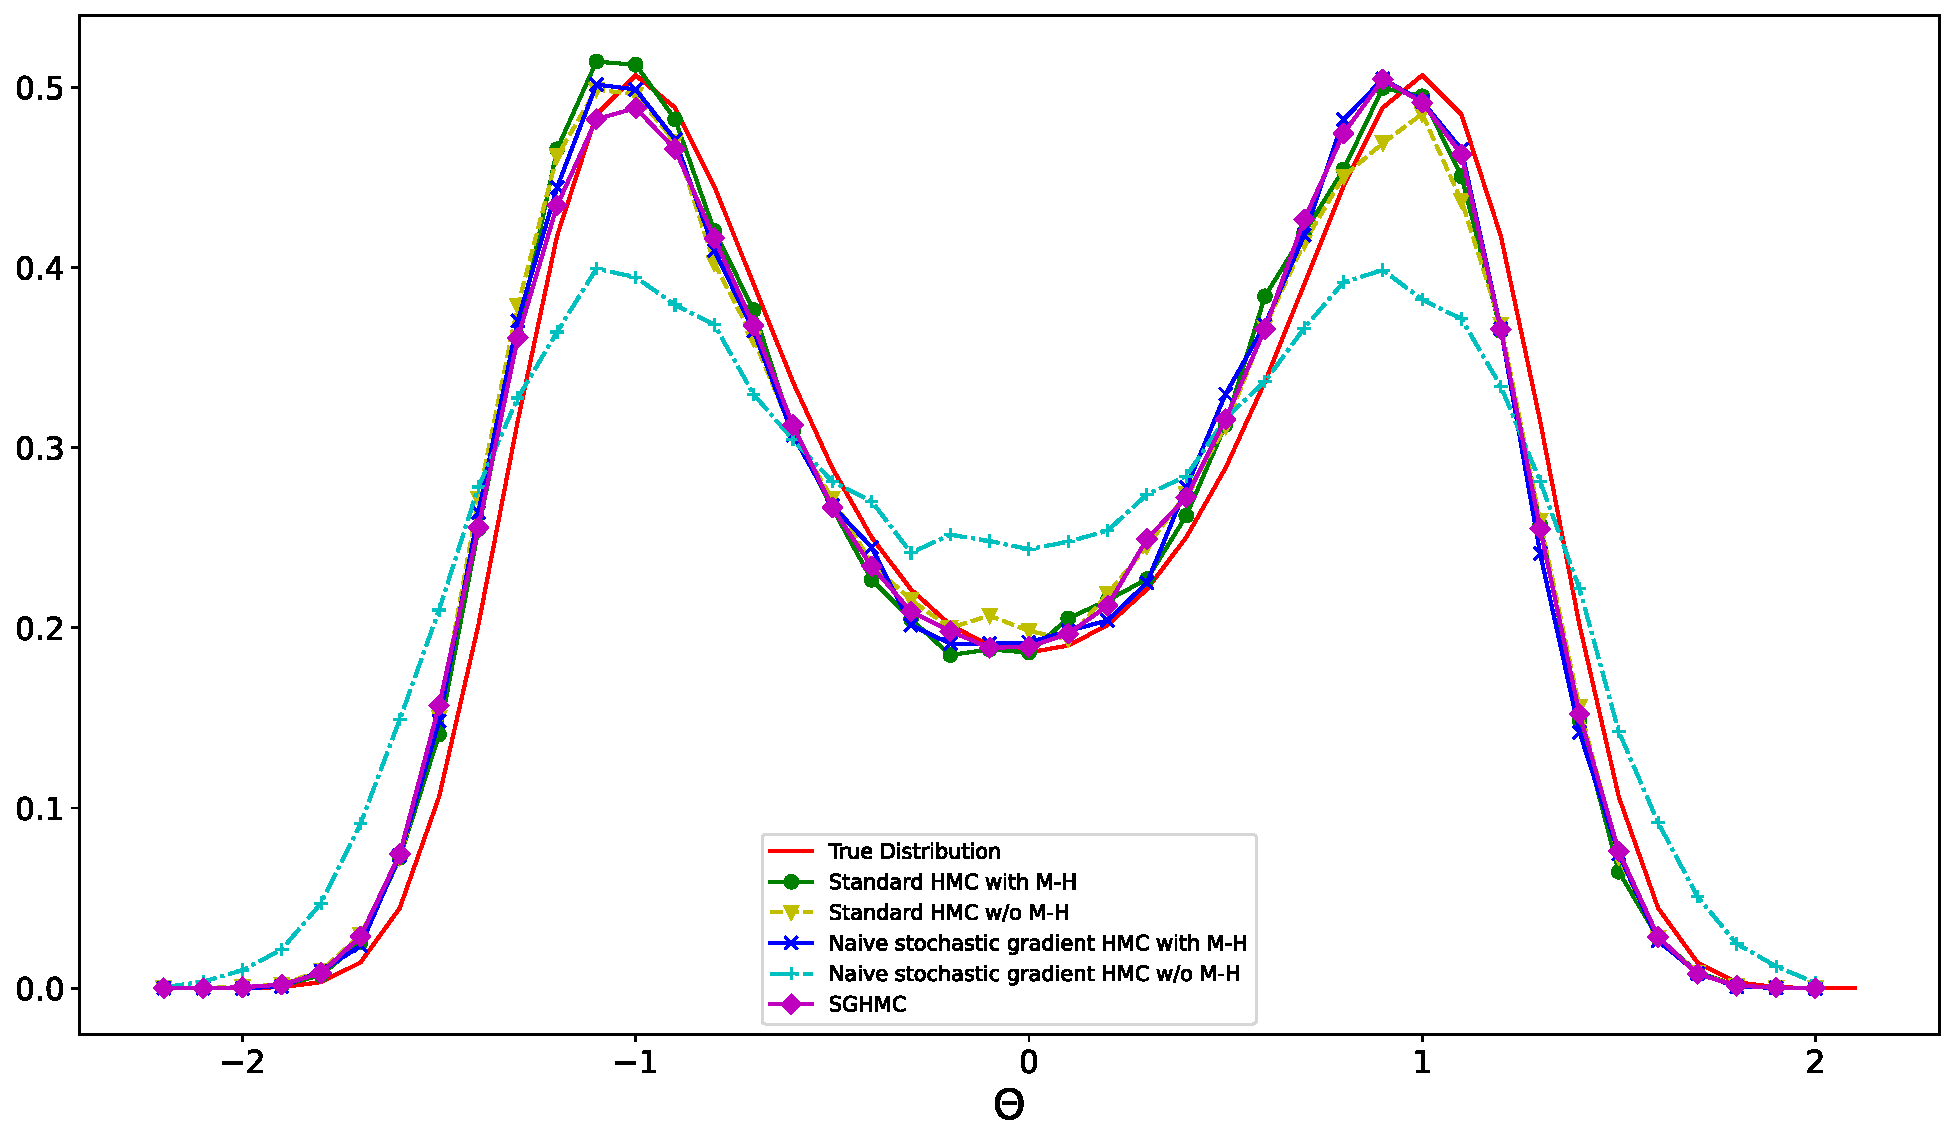
\includegraphics[width=.9\linewidth]{parts/Images/fig1a.pdf}
  \caption{Distributions of different sampling algorithms for the target function $U(\theta) = -2\theta^2 + \theta^4$}
  \label{fig1a}
  \label{fig:demo1}
\end{figure}
\begin{figure}[h!]
  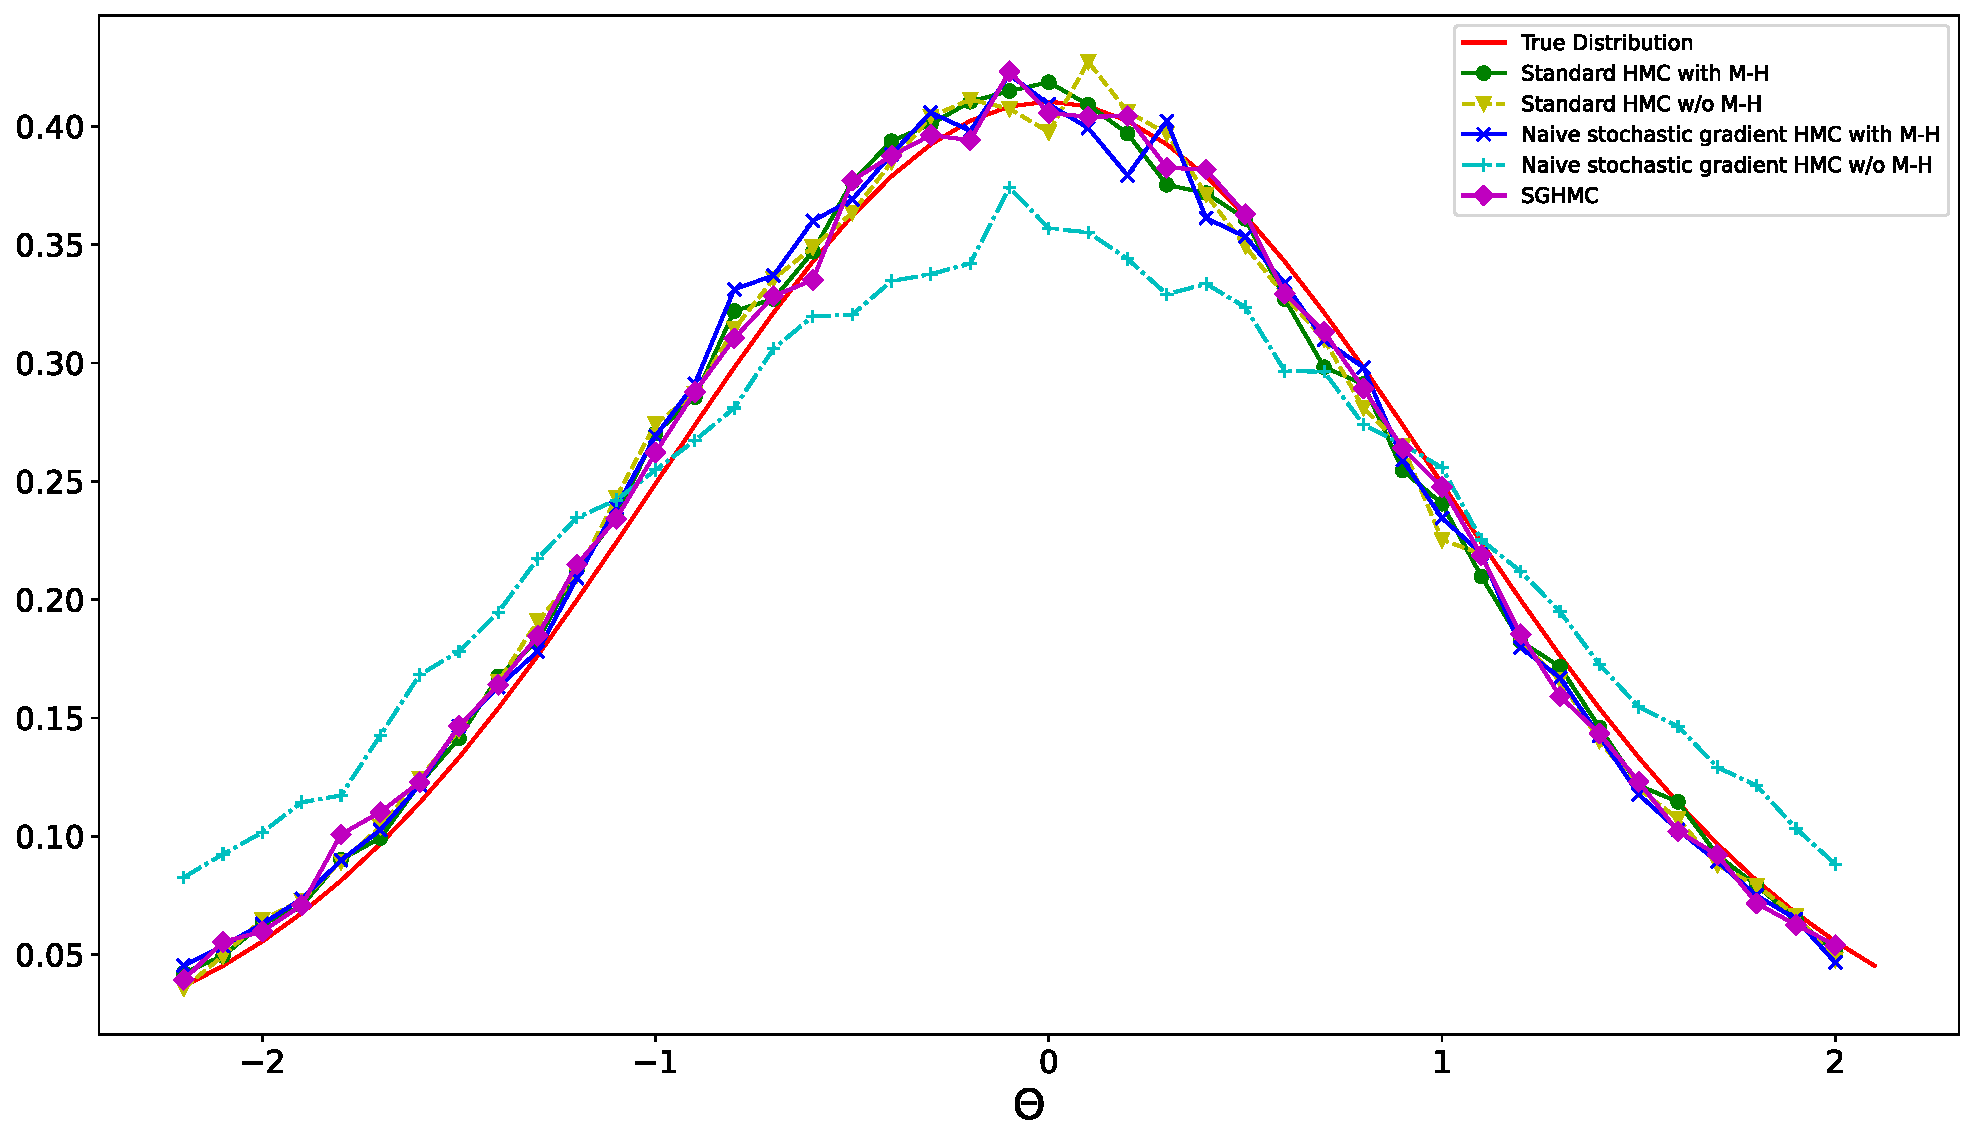
\includegraphics[width=.9\linewidth]{parts/Images/fig1b.pdf}
  \caption{Distributions of different sampling algorithms for the target function $U(\theta) = \frac{1}{2}\theta^2$}
  \label{fig:demo2}
\end{figure}

It can be seen that both HMC algorithms perform well, as does Naïve SGHMC with MH corrections. However, as we already discussed these two algorithms are computationally demanding when used on large datasets. Furthermore, Naïve SGHMC does not converge to the correct distribution, empirically confirming Corollary 3.1 of \cite{sghmc}. On the other hand, SGHMC is fast and maintains the target distribution as its invariant distribution and so can be considered as a useful candidate for scalable Bayesian inference. We note here that our diagram for $U(\theta) = -2\theta^2 + \theta^4$ mirrors that in the paper closely.
\subsubsection*{Experiment 2}

Next we sampled not just $\theta$ using these algorithms, but $(\theta, r)$. Except in the case specified, we did not resample the momentum $r$ here. We plotted the samples found using Hamiltonian Dynamics (HMC), Noisy Hamiltonian Dynamics (Naïve SGHMC), Noisy Hamiltonian Dynamics with momentum resampling (Naïve SGHMC) and Noisy Hamiltonian Dynamics with friction (SGHMC). We used $U(\theta) = \frac{1}{2}\theta^2$, and for the noisy algorithms, as before, we used 
$\nabla \widetilde{U}(\theta) = \nabla U(\theta) + \mathcal{N}(0,4)$. The results are shown in \cref{fig:theta_r_samples}, which closely match those of \cite{sghmc}. Note that there it is said that the samplers were run for 15000 steps, however their plot shows far fewer points. We simulated for 15000 steps and for 360, and decided that the later better illustrated the dynamics and aligned more closely with the original plot.

\begin{figure}[h!]
    \centering
    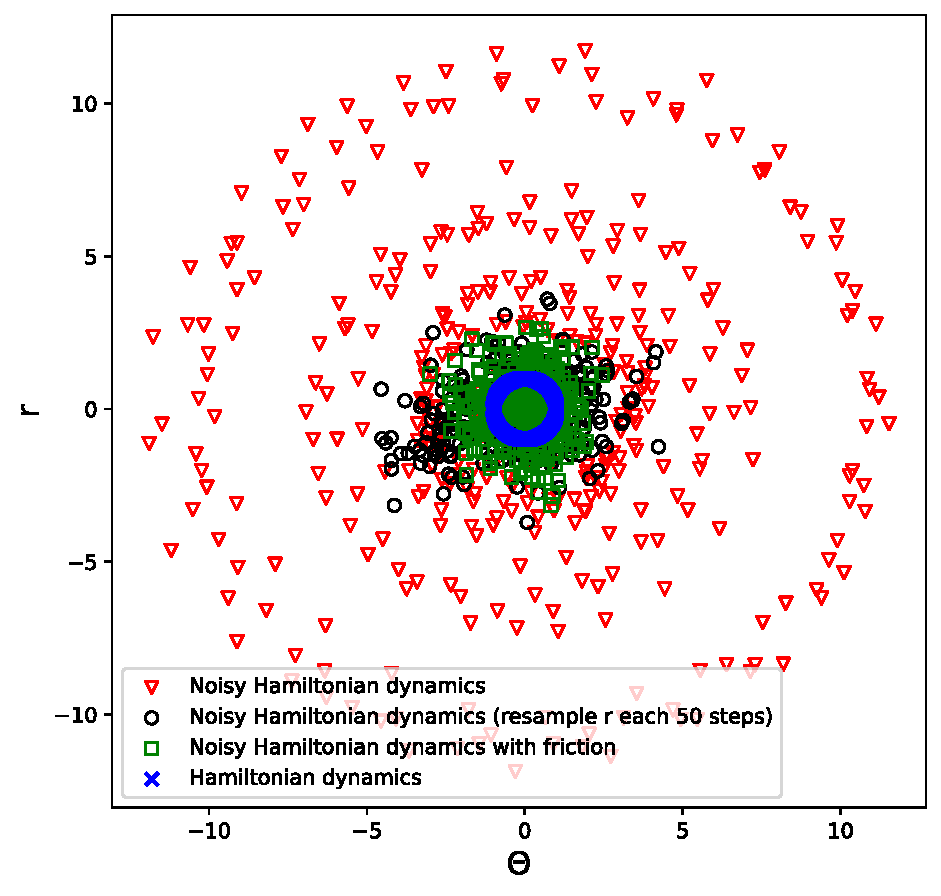
\includegraphics[width=0.9\linewidth]{parts/Images/fig2a.pdf}%
    \caption{Plotting the trajectory of $(\theta, r)$ under various samplers for 360 steps}
     \label{fig:theta_r_samples}%
\end{figure}

These results show that Naïve SGHMC diverges from the true distribution in the samples. This problem is mitigated somewhat when we introduce resampling of $r$ every 50 steps, and is mitigated further if we introduce SGHMC.

\subsubsection*{Experiment 3}

Thirdly, we consider a correlated distribution, as is done in \cite{sghmc}. They note that the strength of HMC is typically in its efficiency in sampling from correlated distributions, and that SGHMC shares this. We replicated the paper's experiment in which they contrast SGHMC and Stochastic Gradient Langevin Dynamics (SGLD) by considering a potential function of $U(\theta)=\frac{1}{2}\theta^T\Sigma^{-1}\theta$, with
$\nabla \widetilde{U}(\theta) = \Sigma^{-1}\theta + \mathcal{N}(0,I)$ with $\Sigma_{11} = \Sigma_{22} = 1$ and correlation $\rho = \Sigma_{12} = 0.9$.  

See \cref{fig:sghmc vs sgld} for the results. The first plot shows 50 samples produced using both algorithms. The second shows the average absolute error of the sample covariance against autocorrelation time (for more details see \cite{sghmc}.


\begin{figure}[h!]
  \begin{subfigure}{.5\textwidth}
  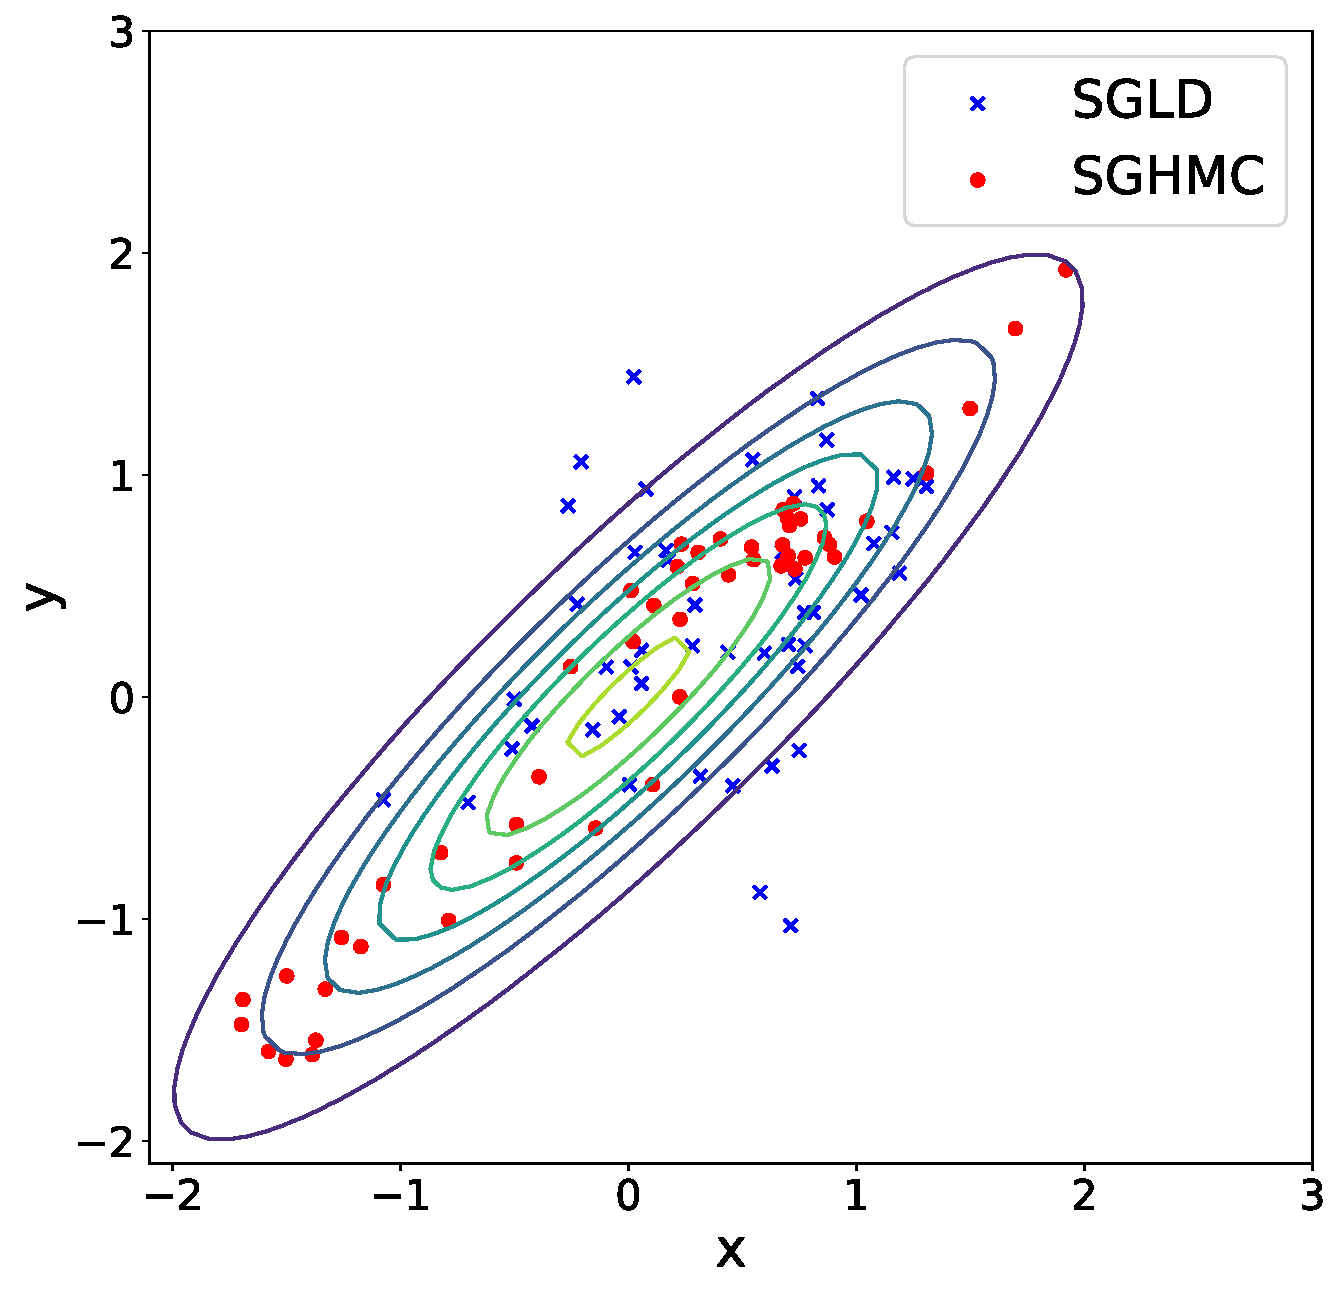
\includegraphics[width=.95\linewidth]{parts/Images/fig3b.pdf}
  \caption{First 50 samples of SGHMC and SGLD}
  \end{subfigure}
  \begin{subfigure}{.5\textwidth}
  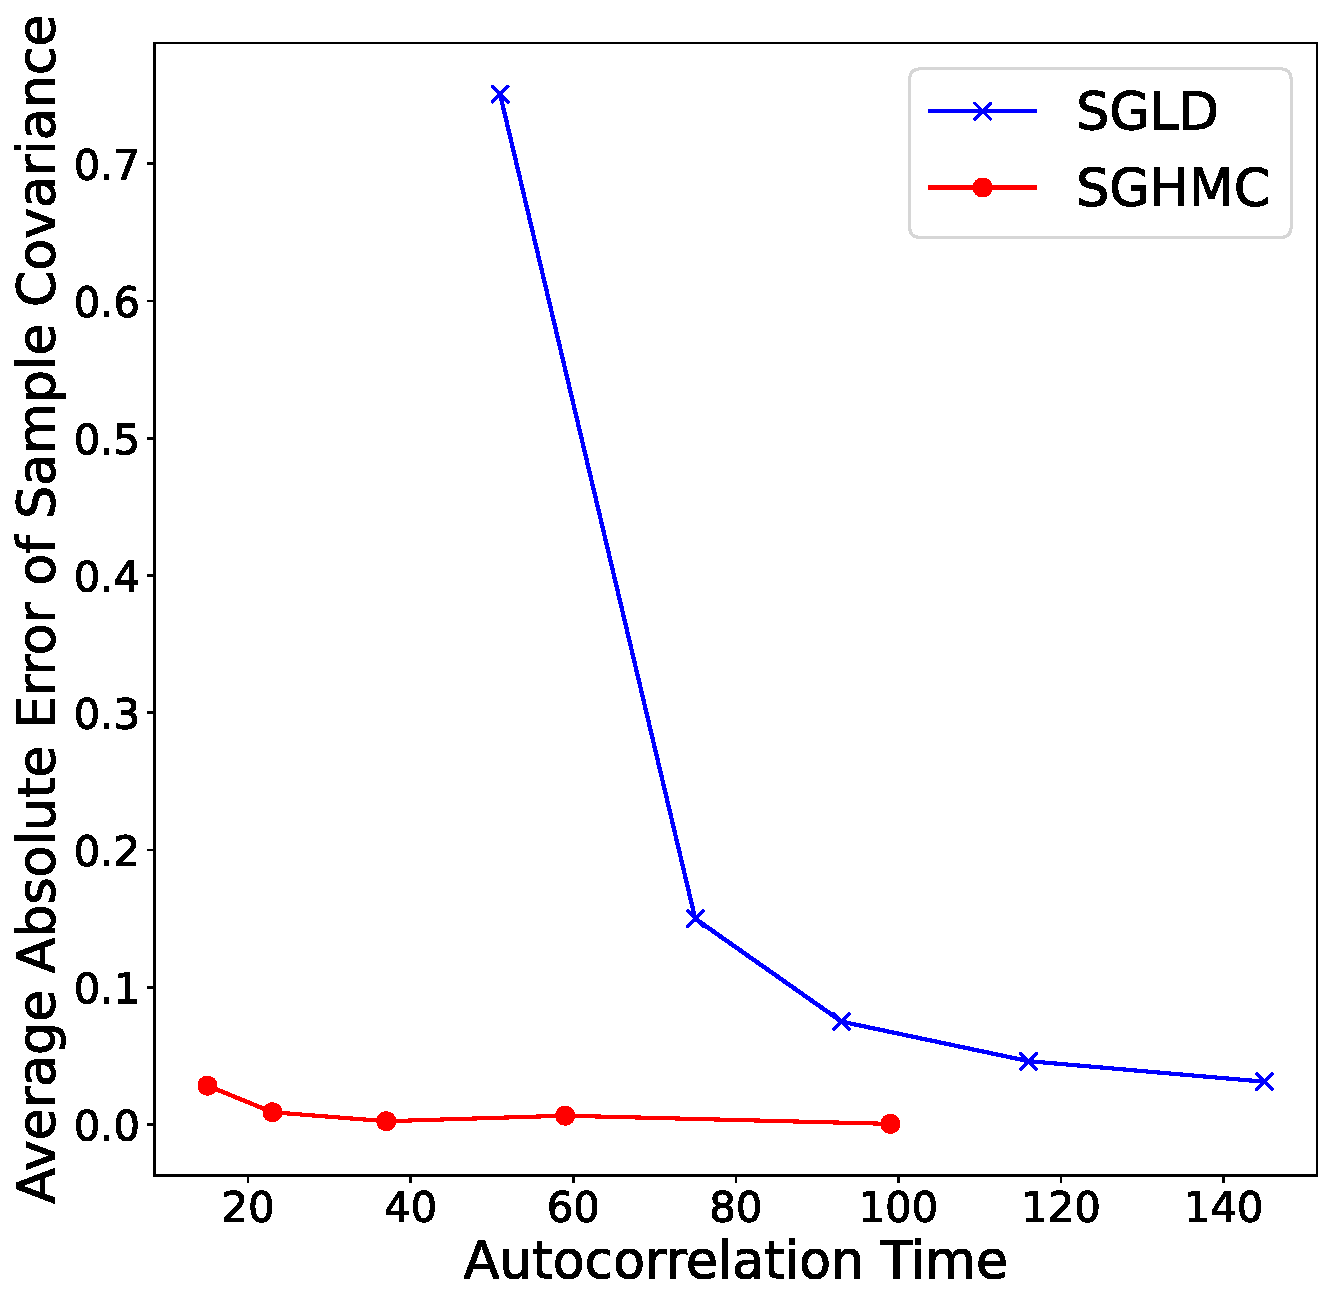
\includegraphics[width=.95\linewidth]{parts/Images/fig3a.pdf}
  \caption{Autocorrelation time versus estimation error for the five setting}
  \end{subfigure}%
  \caption{Contrasting sampling of a bivariate Gaussian with correlation using SGHMC versus SGLD.}
  \label{fig:sghmc vs sgld}
\end{figure}

We can see from this that samples from SGHMC quickly become uncorrelated, which is not true in SGLD. While both SGHMC and SGLD accurately sample from the posterior, SGHMC needs fewer samples to fully explore the posterior distribution. Therefore SGHMC has a faster mixing time than SGLD.


\subsection{Bayesian Neural Networks for Classification}

For the Bayesian neural network (BNN) MNIST classification we actually used the reparameterisation of SGHMC described in the section ``Connection to SGD with Momentum'' of \cite{sghmc}. The SGHMC algorithm is reframed in terms of learning rate and momentum decay, and simulates the following dynamics instead:
$$\begin{cases}
\delta \theta = v\\
\delta v = - \eta \nabla \wt{U}(\theta) - \alpha v + \mathcal{N}(0, 2(\alpha - \wh{\beta}) \eta)
\end{cases}
$$
where $\eta = \epsilon^2 M^{-1}, \alpha = \epsilon M^{-1}C, \wh{\beta} = \eta M^{-1}\wh{B}$. In all our experiments in this section we set the mass matrix $M $ to the identity, and the noise model $\wh{\beta} = \wh{B} = 0$. Other than the architecture of the BNN there are now only 3 hyperparameters for SGHMC, the learning rate $\eta$, the momentum decay $\alpha$ and the batch size $|\wt{\D}|$, in all our experiments we fixed $|\wt{\D}| = 500$ which follows from \cite{sghmc}.

To build on top of the work in \cite{sghmc} we implemented learning rate annealing for SGLD, and following \cite{sgld} we performed a weighted average of our samples using the learning rate. With $f_\theta(\textbf{x})$ being our softmax vector formed from a classifier with parameters $\theta$ with input $\textbf{x}$, we did this as follows:
$$\mathbb{E}[f_{\theta_T}(\textbf{x})] \approx \frac{\sum^T_{t=1} \eta_t f_{\theta_t}(\textbf{x})}{\sum^T_{t=1} \eta_t}$$

Note that as $f$ is a classifier we can ignore the denominator. Our BNN followed the same architecture as in \cite{sghmc}, that is one linear layer with 100 hidden units followed by ReLU activation followed by another linear layer and a log softmax for multi-class classification. The weights and biases for both linear layers are sampled from univariate standard normal distributions, but the Pyro method \texttt{to\_event()} declares dependence between the parameters. 

Our implementations of SGD and SGD with momentum are meant to be used directly with Pyro, and so Gaussian priors on the weights and biases is equivalent to L2 regularization in the non-Bayesian paradigm. We experimented with regularization strengths of $\lambda \in \{0.1, 1.0, 10.0\}$ and found $\lambda = 1.0$ to be the most effective. Additionally we implemented weight decay for both SGD and SGD with momentum but found that this didn't improve anything in this setting.

For the momentum based algorithms, SGHMC and SGD with momentum, we tried $\eta \in \{1.0, 2.0, 4.0, 8.0 \} \times 10^{-6}$, and $\alpha \in \{0.1, 0.01, 0.001 \}$. For SGHMC the best configuration was $\eta = 2.0\times 10^{-6}, \alpha=0.01$, and for SGD with momentum the best configuration was $\eta = 1.0\times 10^{-6}, \alpha=0.01$.

For SGLD and SGD, we tried $\eta \in \{1.0, 2.0, 4.0, 6.0\} \times 10^{-5}$, for SGLD we also tried learning rate annealing but it proved not to make much of a difference in this setting so we ignored it in the end. The best configuration for SGLD was $\eta = 4.0\times 10^{-5}$, and for SGD the best configuration was $\eta = 1.0\times 10^{-5}$.

For MNIST we ran each of the algorithms for 800 epochs with 50 warmup epochs. For the sampling algorithms the warmup epochs allow the sampler to reach the posterior distribution, and then we perform Bayesian averaging over the set $\Theta$, which consists of all of the sampled $\theta$. We then report the test error of this method. Bayesian averaging is described in Section II of \cite{hands-on-bnn} and is performed as follows:
$$\mathbf{\hat p} = \sum_{\theta_i \in \Theta} f_{\theta_i} (\mathbf{x}) \qquad ; \qquad \mathbf{\hat y} = \text{argmax}_{i} \{ p_i \in \mathbf{\hat p} \}$$
For the optimization algorithms we take the most recent sample / set of parameters as a point estimate and report the test error.  \cref{fig:MNIST} presents our results.
\begin{figure}[h!]
\centering
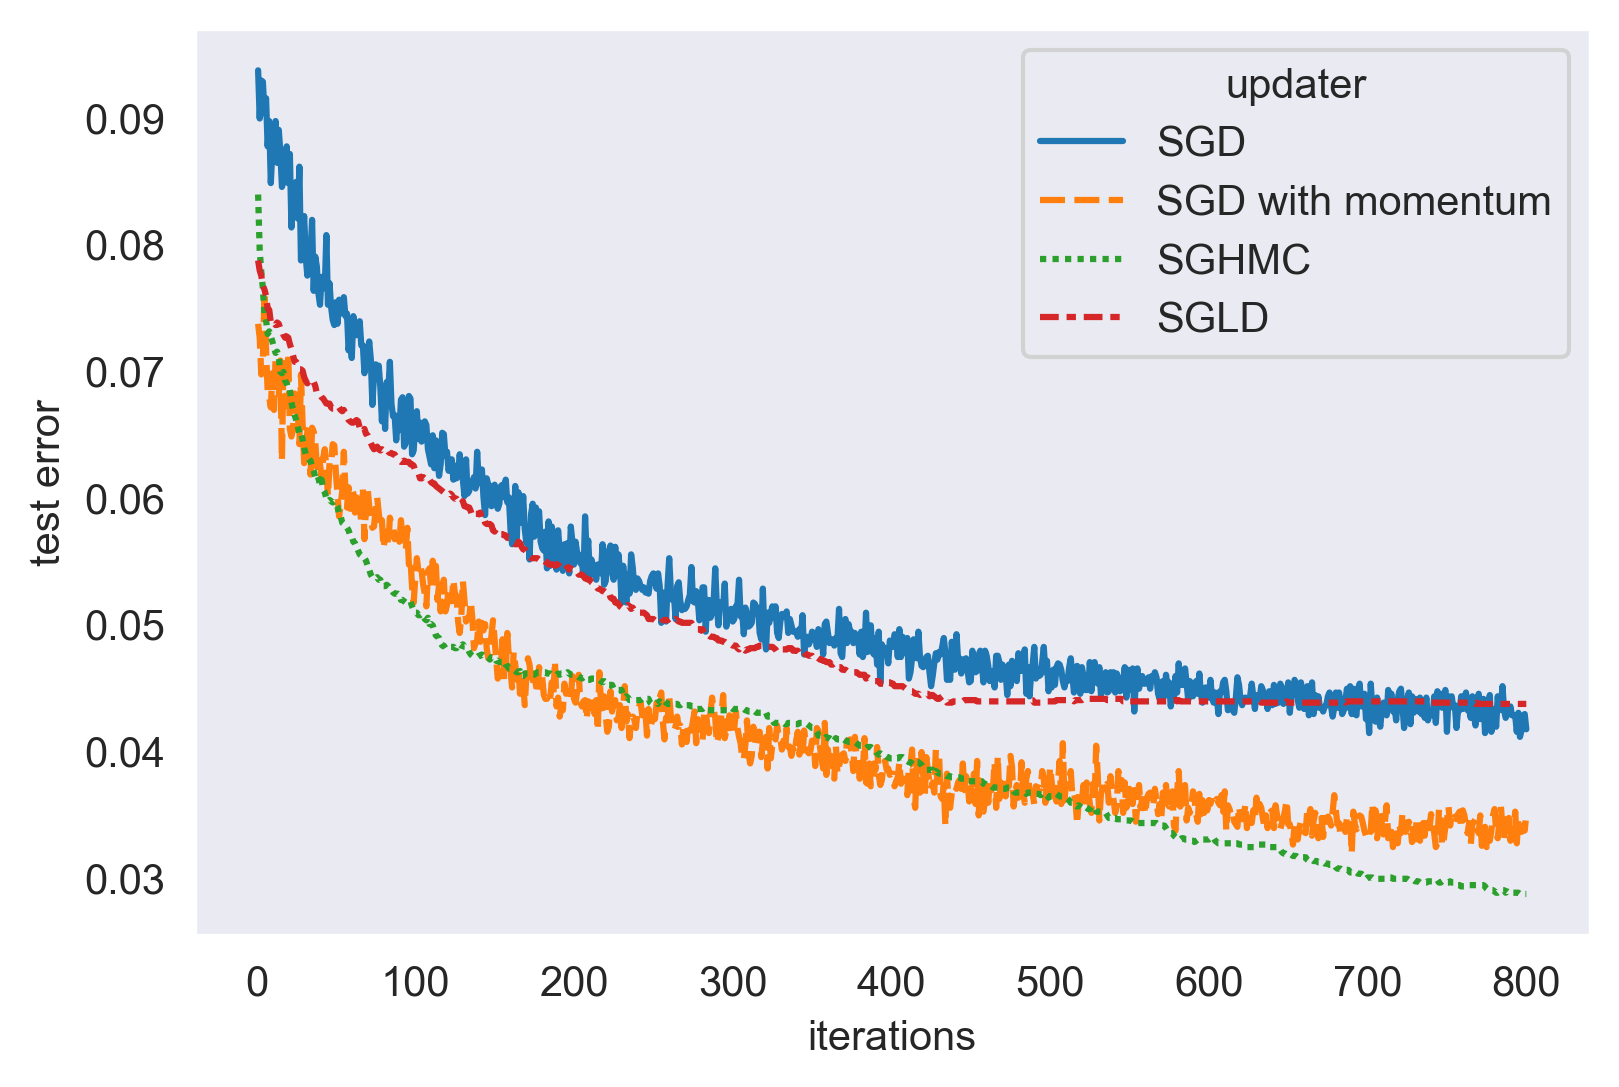
\includegraphics[width=100mm]{parts/Images/MNIST.png}
\caption{Reproducing the MNIST classification experiment from \cite{sghmc}; SGHMC ($\eta = 2.0\times 10^{-6}, \alpha=0.01, \texttt{resample\_n} =0$ ), SGLD ($\eta = 4.0\times 10^{-5}$), SGD ($\eta = 1.0\times 10^{-5}$), SGD with momentum ($\eta = 1.0\times 10^{-6}, \alpha=0.01$)}
\label{fig:MNIST}
\end{figure}
The results we get from MNIST classification align very closely with those in \cite{sghmc} and so we come to the same conclusion; the need for scalable and efficient Bayesian inference algorithms. The key benefit of BNNs is that we are not overconfident on out-of-distribution examples, \cref{fig:B} illustrates that we still maintain this property when using SGHMC to approximately sample from the posterior distribution. We additionally conducted a brief comparison between Variational Inference (VI) and SGHMC in this setting, \cref{fig:VI} outlines our findings.
\begin{figure}[h!]
\centering
\begin{subfigure}{.5\textwidth}
  \centering
  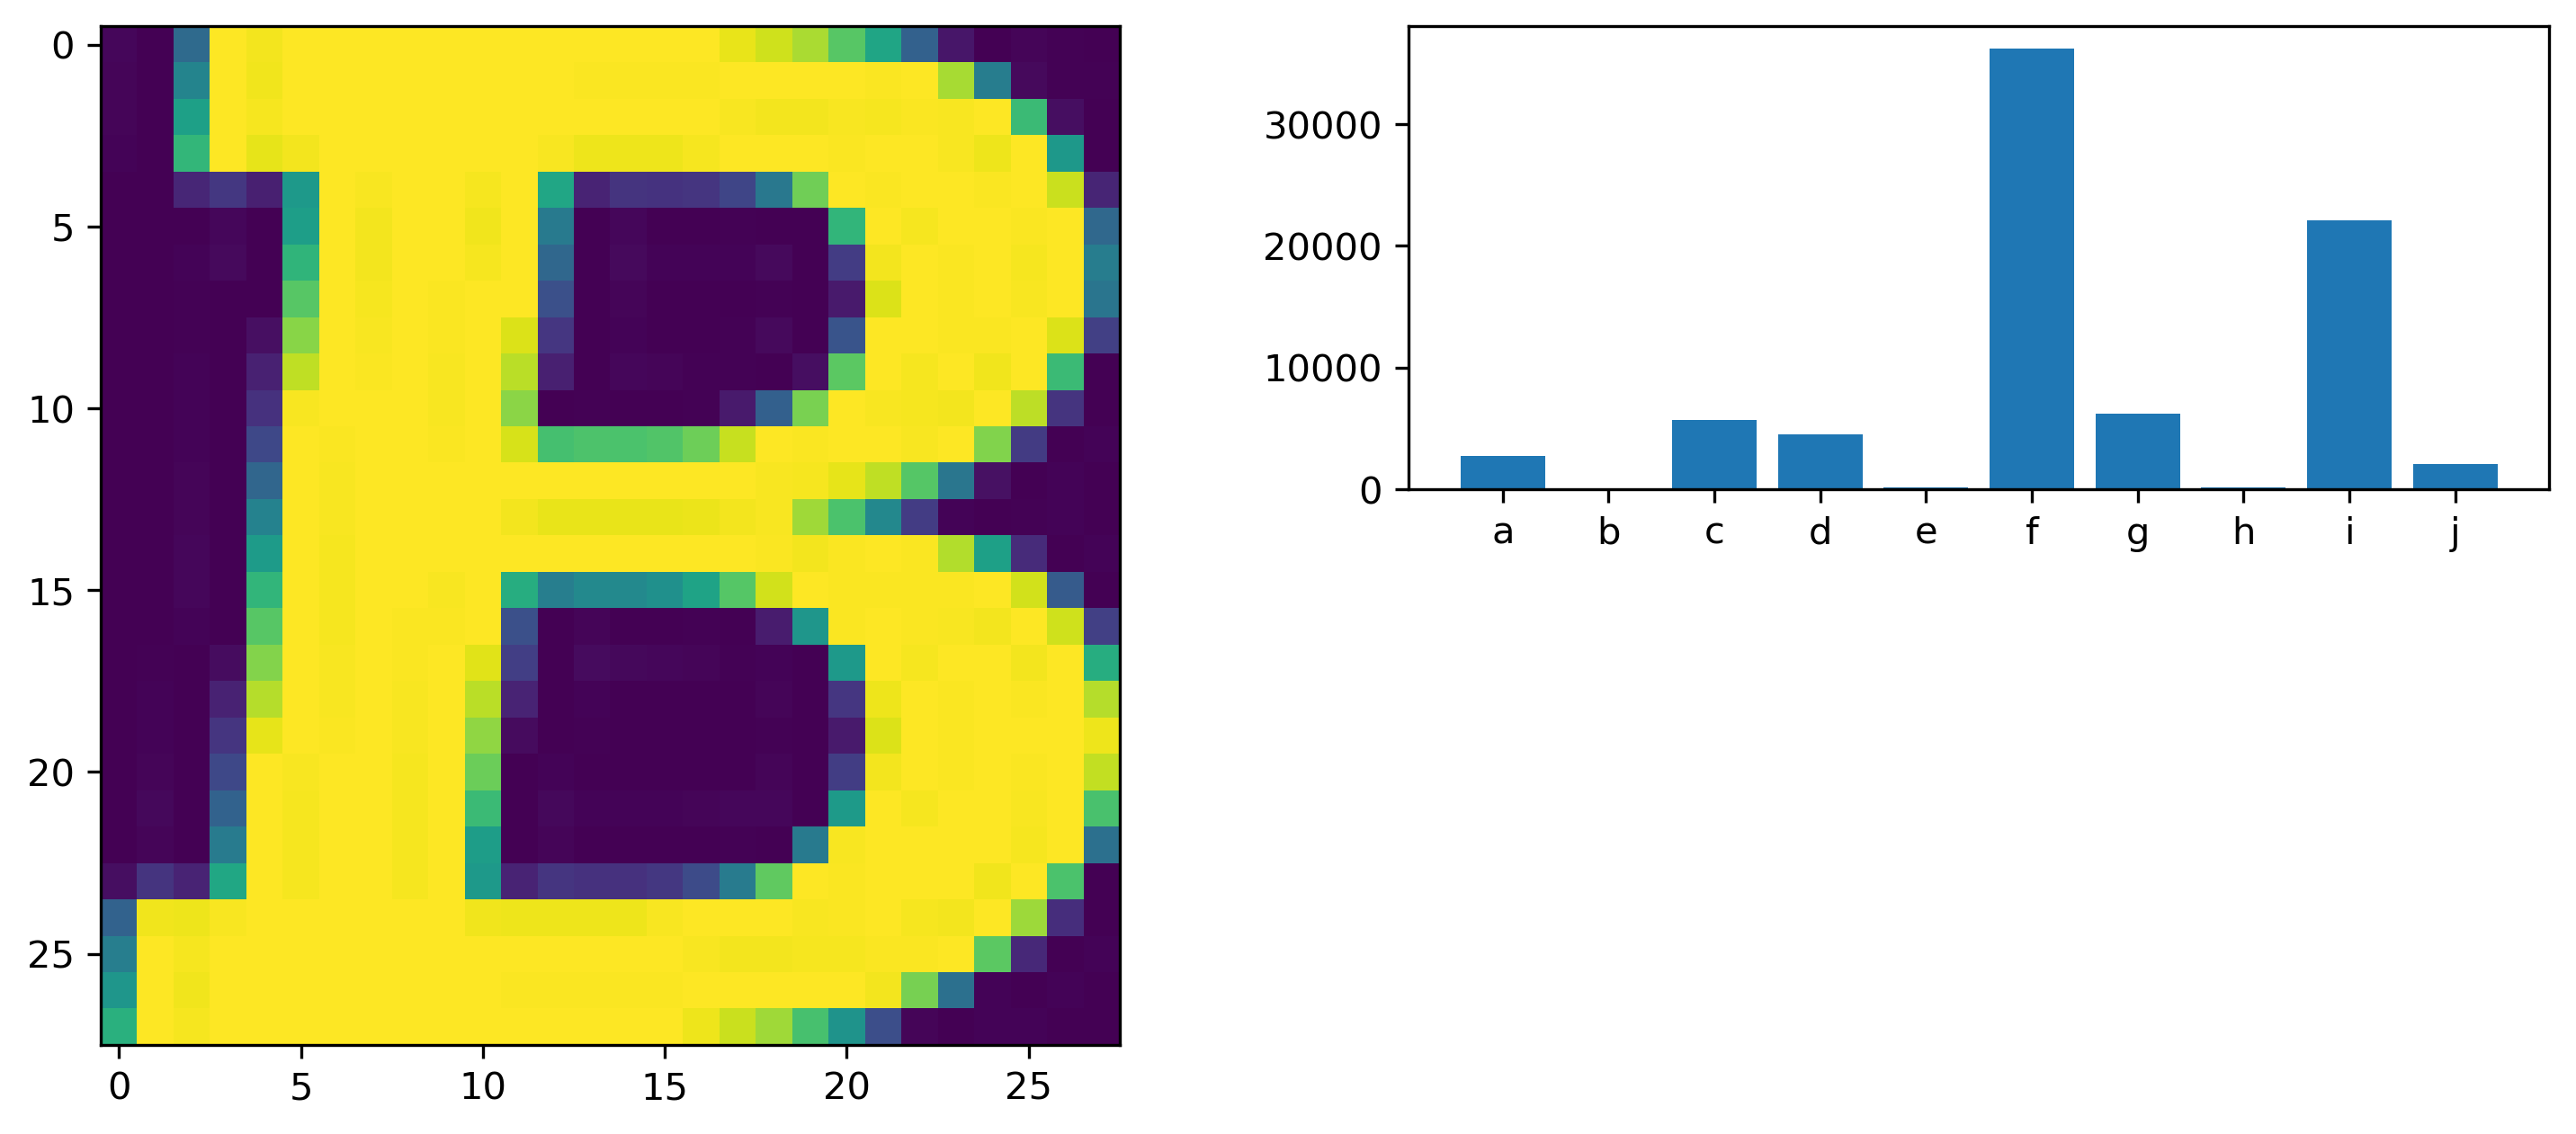
\includegraphics[width=.95\linewidth]{parts/Images/B.png}
  \caption{Uncertainty in out-of-distribution examples}
  \label{fig:B}
\end{subfigure}%
\begin{subfigure}{.5\textwidth}
  \centering
  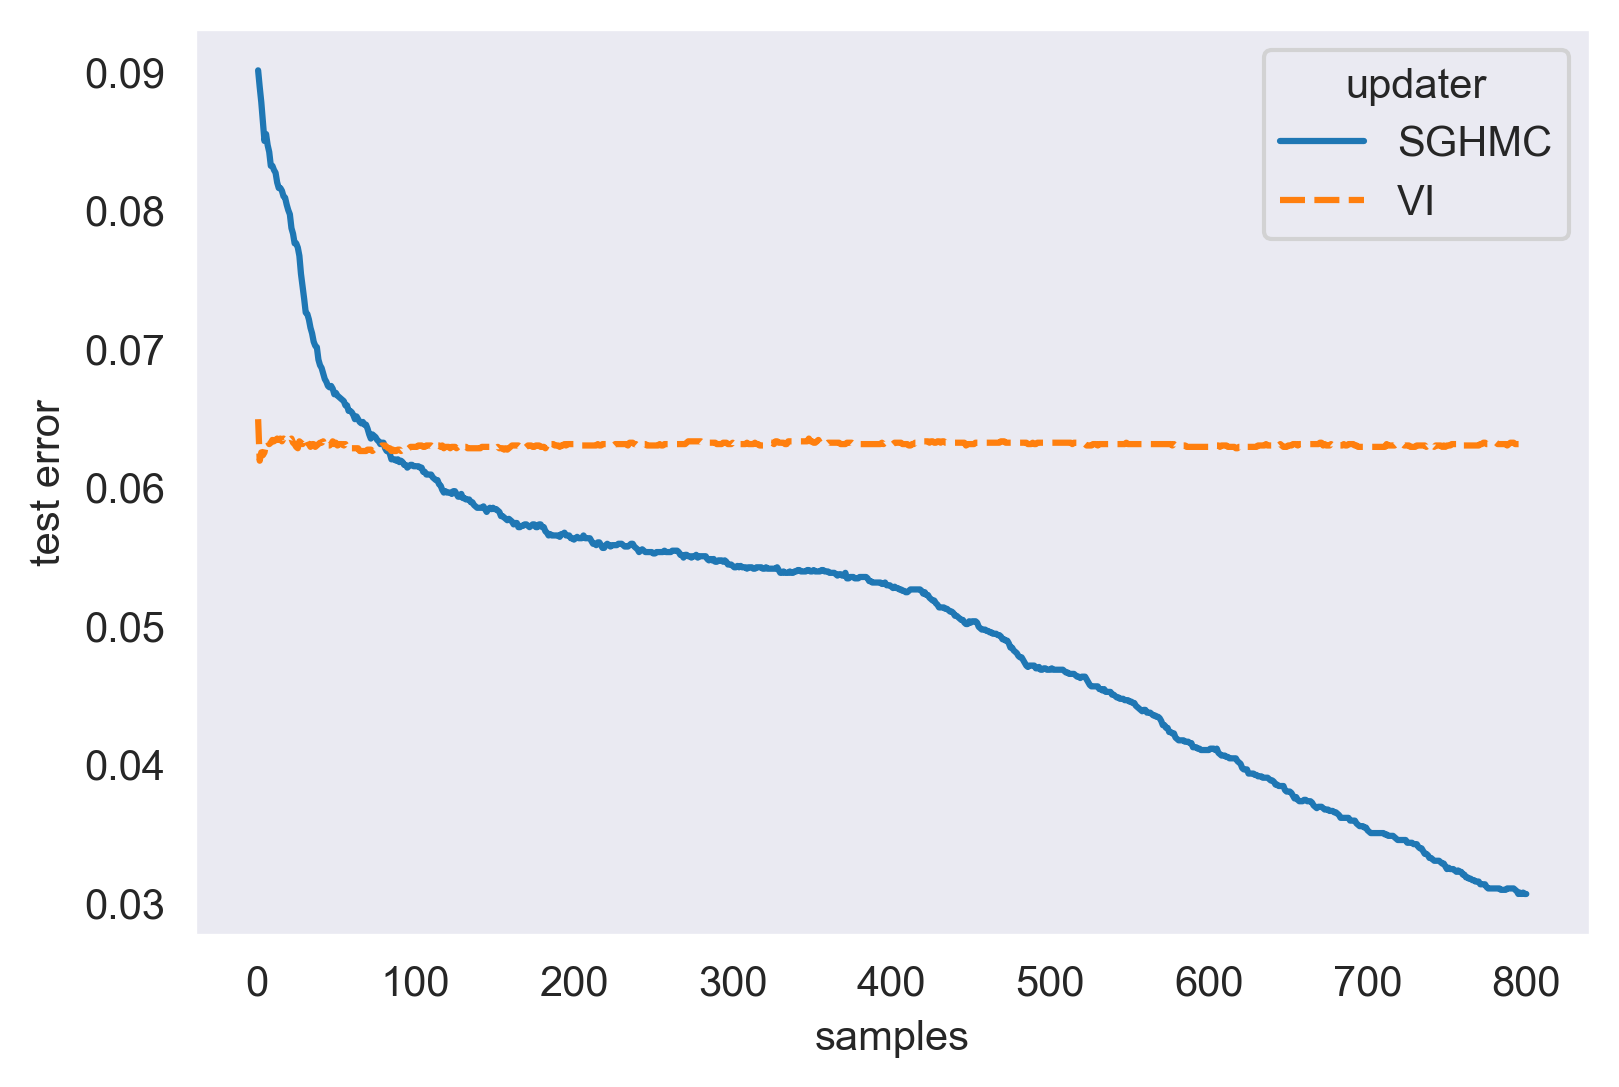
\includegraphics[width=.95\linewidth]{parts/Images/VI_SGHMC.png}
  \caption{VI and SGHMC on MNIST}
  \label{fig:VI}
\end{subfigure}
\caption{{\bf Left} (a) illustrates that we get uncertainty estimates on out-of-distribution examples. {\bf Right} (b) compares VI (Renyi ELBO, $\alpha = 0.01$, \texttt{num\_particles} $= 2$) and SGHMC ($\eta = 2.0\times 10^{-6}, \alpha=0.01, \texttt{resample\_n} =0$) on MNIST. For VI we draw 80000 samples from the variational posterior $q_{\phi}$ and report the test error by Bayesian averaging. For SGHMC we do the same, except we are approximately sampling from the true posterior $p(\theta \: | \mathcal{D} \:)$.}
\label{fig:demo}
\end{figure}
The initial results suggest that SGHMC performs better than VI in this setting, although this is not the full picture. Once VI fits the variational posterior distribution $q_{\phi}$ as closely as possible to the true posterior it takes only hundreds of samples to characterise $q_{\phi}$, whereas SGHMC requires several more samples to characterise the true posterior. In practice storing thousands of parameterisations of the same NN is very costly and so this is probably why VI is a more popular choice for Bayesian inference. 

We conclude this section by demonstrating our algorithms can be applied to other datasets and more complicated models, \cref{fig:fashionMNIST} presents the results of running the same BNN architecture on FashionMNIST, and \cref{fig:CIFAR10} demonstrates that our implementation of SGHMC can be used with convolutional neural networks (CNNs).
\begin{figure}[h!]
\centering
\begin{subfigure}{.5\textwidth}
  \centering
  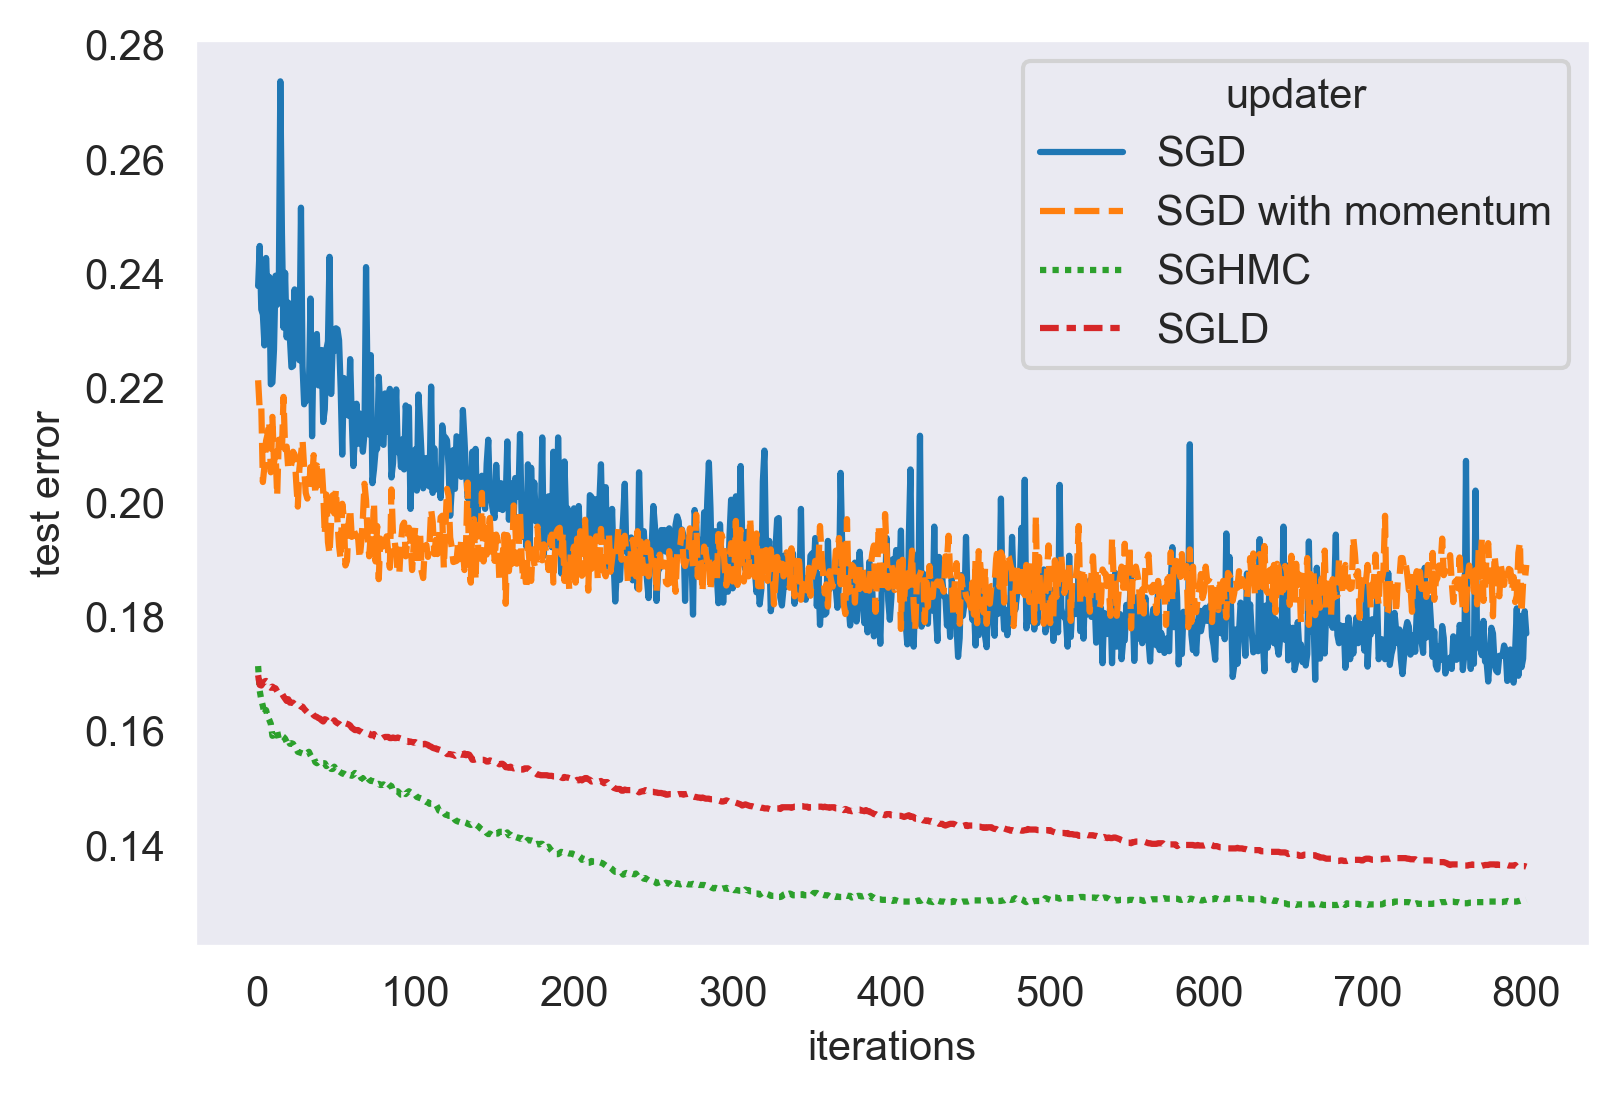
\includegraphics[width=.95\linewidth]{parts/Images/fashion-mnist.png}
  \caption{Experiment on FashionMNIST}
  \label{fig:fashionMNIST}
\end{subfigure}%
\begin{subfigure}{.5\textwidth}
  \centering
  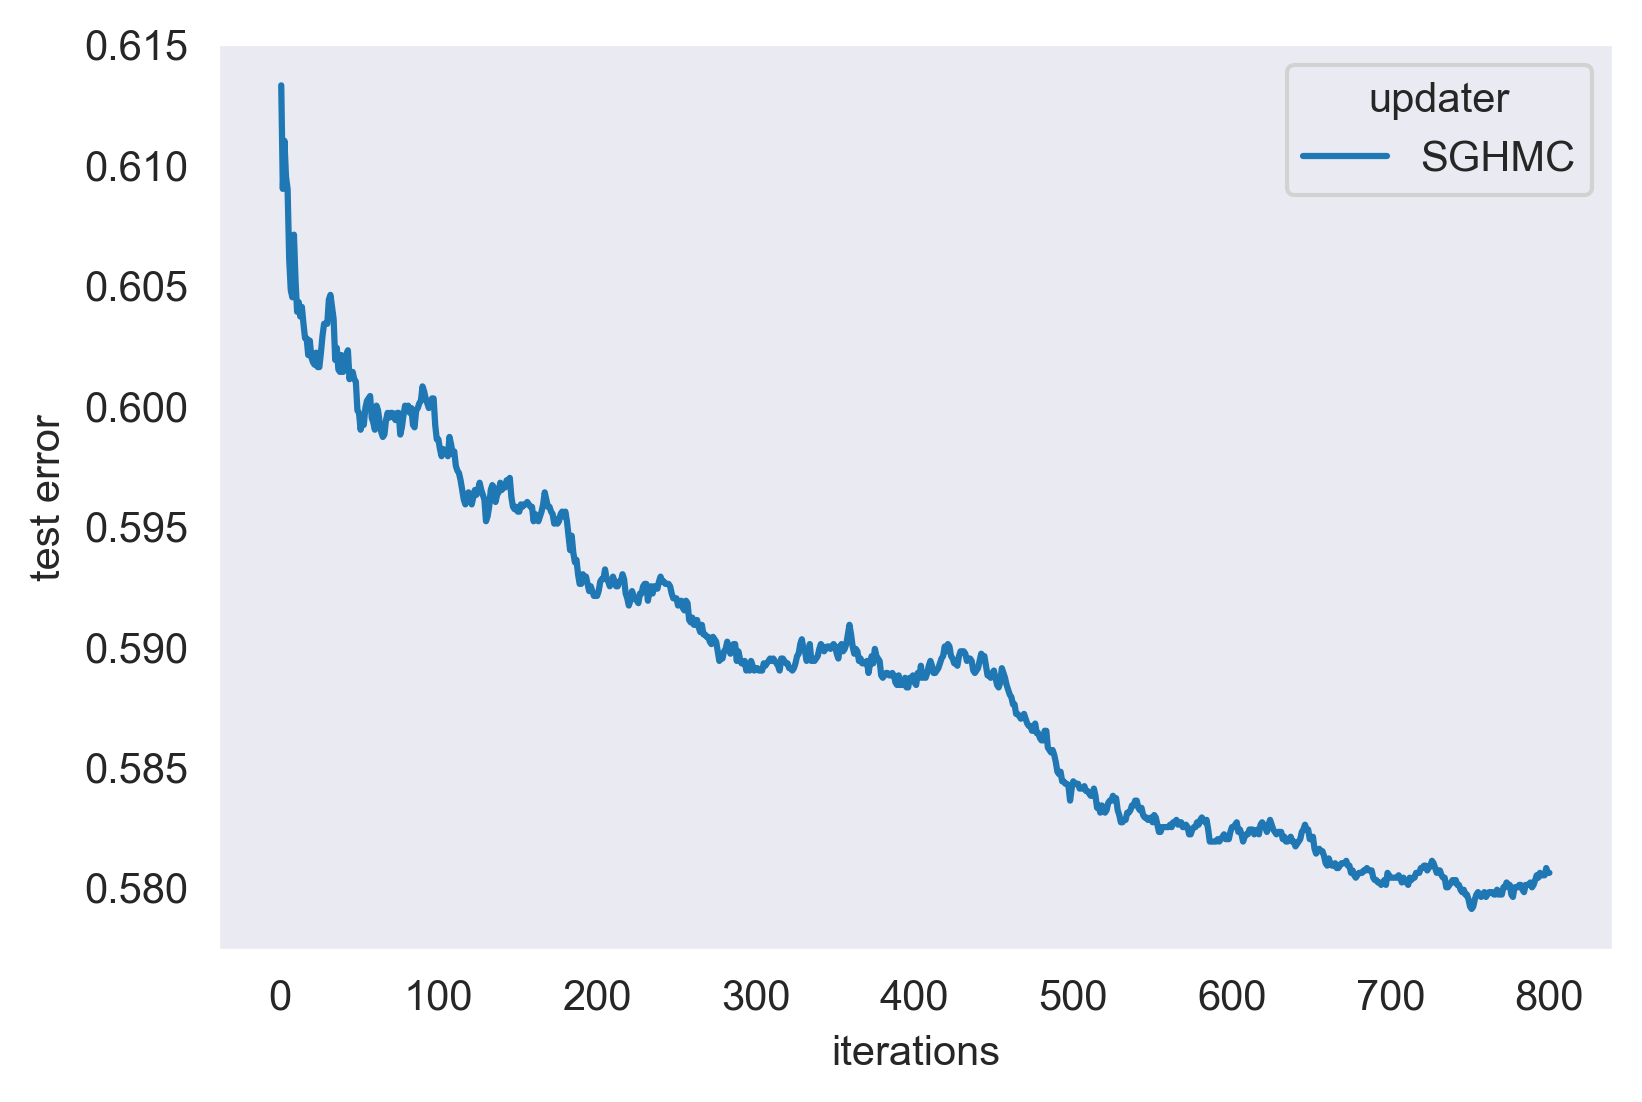
\includegraphics[width=.95\linewidth]{parts/Images/CIFAR10.png}
  \caption{Convolutional BNN on CIFAR10}
  \label{fig:CIFAR10}
\end{subfigure}
\caption{{\bf Left} (a) FashionMNIST classification; SGHMC ($\eta = 1.0\times 10^{-6}, \alpha=0.01, \texttt{resample\_n} =0$ ), SGLD ($\eta = 1.0\times 10^{-5}$), SGD ($\eta = 1.0\times 10^{-5}$), SGD with momentum ($\eta = 1.0\times 10^{-6}, \alpha=0.01$); \texttt{warmup\_epochs} $= 100$. {\bf Right} (b) Convolutional BNN with 2 convolutional layers, batch norm, max pooling and tanh activations followed by two Bayesian linear layers with tanh activation;  SGHMC ($\eta = 1.0\times 10^{-6}, \alpha=0.01, \texttt{resample\_n} =0$ ) ; \texttt{warmup\_epochs} $= 150$.}
\label{fig:other-datasets}
\end{figure}

\end{document}

	\section{NUTS}
\subsection{The Basic Algorithm}

In our current description of the SGHMC algorithm we have the user-defined hyperparameter $m$, the number of steps iterated over before we take a sample. If this number is too small, our samples will be correlated, and hence successive samples would appear to follow a random walk, and we would get slow mixing times. We demonstrate this behaviour by training 3 versions of SGHMC with $m=1,3,5$ (with $\epsilon m$ fixed). The learning curves below in figure \ref{num_steps} show that increasing $m$ increases the speed with which SGHMC reaches low error rates.

\begin{figure}[h!]
\centering
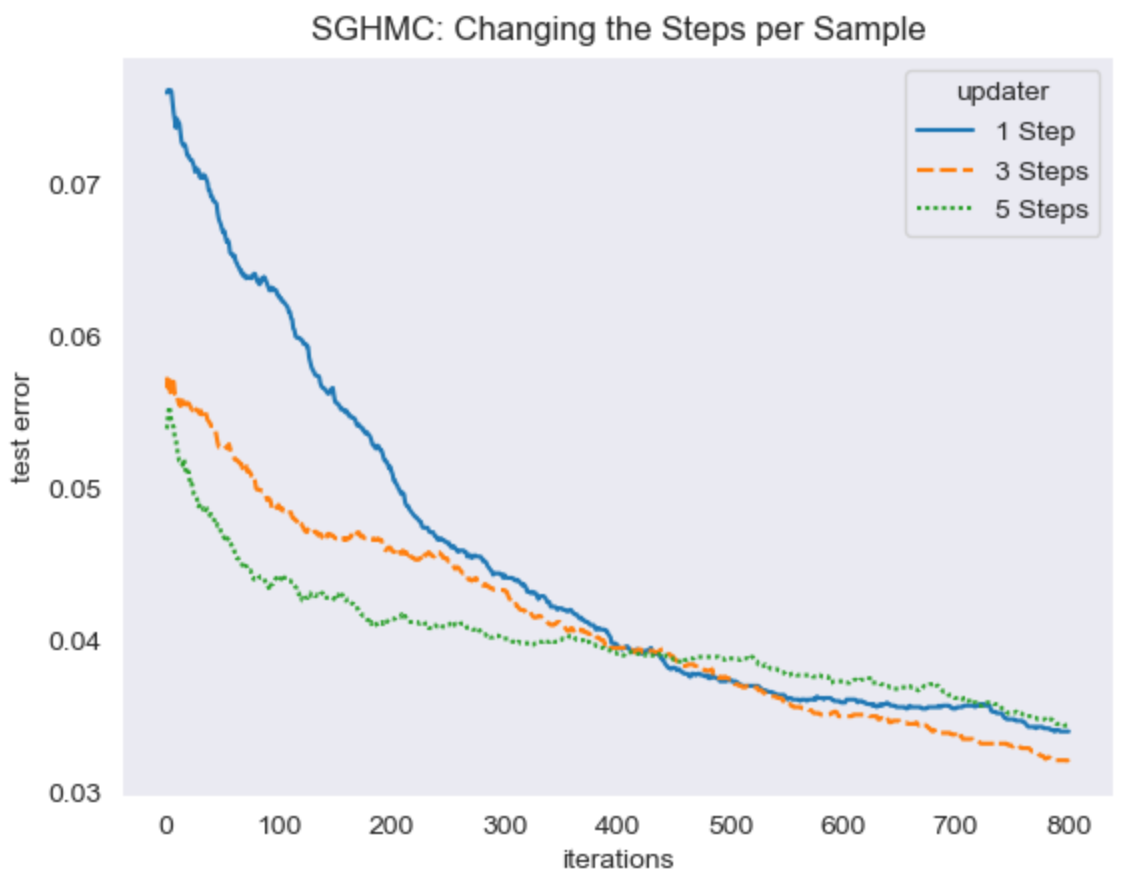
\includegraphics[width=100mm]{parts/Images/changing_num_steps.png}
\caption{Changing the number of steps per sample. Each agent was run for 100 warmup epochs.}
\label{num_steps}
\end{figure}

However, if $m$ is too large we waste computational power, as we continue to step through time even though each sample is already independent of the last. We would like to set $m$ to its optimal value.

Hoffman and Gelman introduce the algorithm NUTS in their paper ``The No-U-Turn Sampler: Adaptively Setting Path Lengths in Hamiltonian Monte Carlo'' \cite{nuts}. In its basic form this algorithm removes the need for a user to input a value for $m$ in the standard HMC implementation. We converted this NUTS algorithm from being based on HMC to being based on SGHMC, and investigated its power. We will begin by presenting the high level overview of the original NUTS algorithm for HMC sampling.

The key idea is the concept of a `U-Turn'. This is the point at which the samples of $\theta$ start to get closer to the initial value of $\theta$, rather than away from it. This marks the point at which further steps will likely only waste computational power. Mathematically, for current position $\theta$, initial position $\theta_0$ and momentum $r$, this corresponds to the time at which:
$$ \frac{d}{dt} |\theta - \theta_0|^2 = 2(\theta - \theta_0)\cdot\frac{d\theta}{dt} = 2(\theta - \theta_0)\cdot r< 0$$
where we use the fact that in the dynamics of HMC (and also SGHMC) we have $\frac{d\theta}{dt} = r$. This simple fact suggests an algorithm in which we draw the sample $\theta$ once we have performed enough steps so that $(\theta - \theta_0)\cdot r< 0$. However this is too simplistic an approach - as HMC is an instance of the Metropolis Hastings algorithm we require the Markov Chain of $\theta$ to be reversible, which is not the case here.

To remedy this problem, NUTS requires keeping track of a set $\mathcal{B}$, which contains all values of $(\theta, r)$ as steps are taken both forward and backwards in time. The values at the earliest and latest times considered across a single trajectory are labelled  $(\theta^-, r^-)$ and $(\theta^+, r^+)$ respectively. NUTS starts from a single $(\theta, r)$ and then steps either forward or backwards one step. It then steps forward or backwards 2 steps, then 4 steps, then 8 steps etc.\@ until a `U-Turn' is seen. A description is as follows:

\begin{enumerate}
    \item Start with an initial $(\theta_0, r_0)$
    \item Set $n\leftarrow1$, $\mathcal{B}\leftarrow \{(\theta_0, r_0)\}$, $(\theta^-, r^-) \leftarrow (\theta_0, r_0) $ and $(\theta^+, r^+) \leftarrow (\theta_0, r_0) $ 
    \item While there is no U-Turn at $(\theta^-, r^-)$ nor at $(\theta^+, r^+)$\\ (ie $(\theta^+ - \theta^-)\cdot r^- \geq 0$ and $(\theta^+ - \theta^-)\cdot r^+ \geq 0$): 
    \begin{enumerate}
        \item Choose to go \textit{forwards} or \textit{backwards} in time, each
        with probability $\frac{1}{2}$.

        \item If \textit{forwards}:
        \begin{enumerate}
            \item $(\theta, r) \leftarrow (\theta^+, r^+)$.
            \item Repeat $n$ times:
            \begin{enumerate}
                \item $(\theta, r) \leftarrow $ Step forward in time from $(\theta, r)$
                \item $\mathcal{B} \leftarrow (\theta, r) \cup \mathcal{B}$
            \end{enumerate}
            \item $(\theta^+, r^+) \leftarrow (\theta, r)$
        \end{enumerate}
        
        \item If \textit{backwards}:
        \begin{enumerate}
            \item $(\theta, r) \leftarrow (\theta^-, r^-)$

            \item Repeat n times:
            \begin{enumerate}
                \item $(\theta, r) \leftarrow $ Step backwards in time from $(\theta, r)$
                \item $\mathcal{B} \leftarrow (\theta, r) \cup \mathcal{B}$
            \end{enumerate}
            \item $(\theta^-, r^-) \leftarrow (\theta, r)$
    
        \end{enumerate}
        \item $n \leftarrow 2n$
    \end{enumerate}
    \item Carefully choose a subset $\mathcal{C} \subseteq \mathcal{B}$. This step is the key to the Markov Chain being reversible, however for clarity's sake we will not go into detail as to how this is done here.
    \item Sample an element of $\mathcal{C}$

\end{enumerate}

The benefit to this algorithm is that it removes the need to set the number of steps performed before we sample, as we keep stepping until a `U-Turn' is seen. We should note here that in the original form of NUTS, the `step' being referred to in $3biiA$ and $3ciiA$ is the step of the HMC algorithm. We edited the NUTS Pyro source code to make it perform SGHMC steps, and we named this SGNUTS.

There were some doubts as to whether the NUTS algorithm would work when using SGHMC steps instead of HMC steps. This was because NUTS requires the ability to step backwards in time, while an SGHMC step includes an injection of stochastic noise. As there is no action that undoes this injection, there was a worry that the backwards step through time in NUTS would become a problem. We explain how we attempted to solve this problem at the end of the next section.

\subsection{Implementation of SGNUTS}
To build SGNUTS we started with the Pyro source code for NUTS \cite{nuts_code} which takes the Pyro HMC class as its parent. We altered this to instead inherit from our SGHMC class. This required removing step-size adaptation and mass matrix adaptation functionality from NUTS, as our implementation of SGHMC was not able to interface with this. It also required introducing some caching methods into the SGHMC class - to help keep things simple in our original SGHMC class we did this in a new class, named SGHMC\_for\_NUTS. Most importantly, we had to alter the $(\theta,v)$ step update rule which is hardcoded in NUTS. This meant that instead of being the HMC update step it was now the SGHMC update step of:

$$
    \theta \leftarrow 
    \begin{cases}\theta + \epsilon M^{-1}r, & \text{{\textit{forwards step}}}\\
                \theta - \epsilon M^{-1}r,  & \text{{\textit{backwards step}}}

\end{cases}
$$
$$
    r \leftarrow 
    \begin{cases}
                
    r - \epsilon \nabla \tilde{U}(\theta) - \epsilon C M^{-1}r + \mathcal{N}(0,2(C-\hat{B})\epsilon), & \text{{\textit{forwards step}}}\\
   
    r + \epsilon \nabla \tilde{U}(\theta) - \epsilon C M^{-1}r + \mathcal{N}(0,2(C-\hat{B})\epsilon), & \text{{\textit{backwards step}}}\\
 \end{cases}
    $$

In particular, note that there is an injection of stochastic noise and momentum-reducing friction in both the forward steps and the backward steps. This is not ideal, as our backwards step in time does not undo a forward step, which likely breaks the reversibility of the Markov Chain being considered in NUTS. However we investigated this nonetheless.

\subsection{Results} 

We tested the SGNUTS algorithm on the BNNs described earlier. We ran SGNUTS for only 20 warmup epoch and 50 epochs as the code was slower than SGHMC to run. The learning curves were as shown in figure \ref{SGNUTS_results}:

\begin{figure}[h!]
\centering
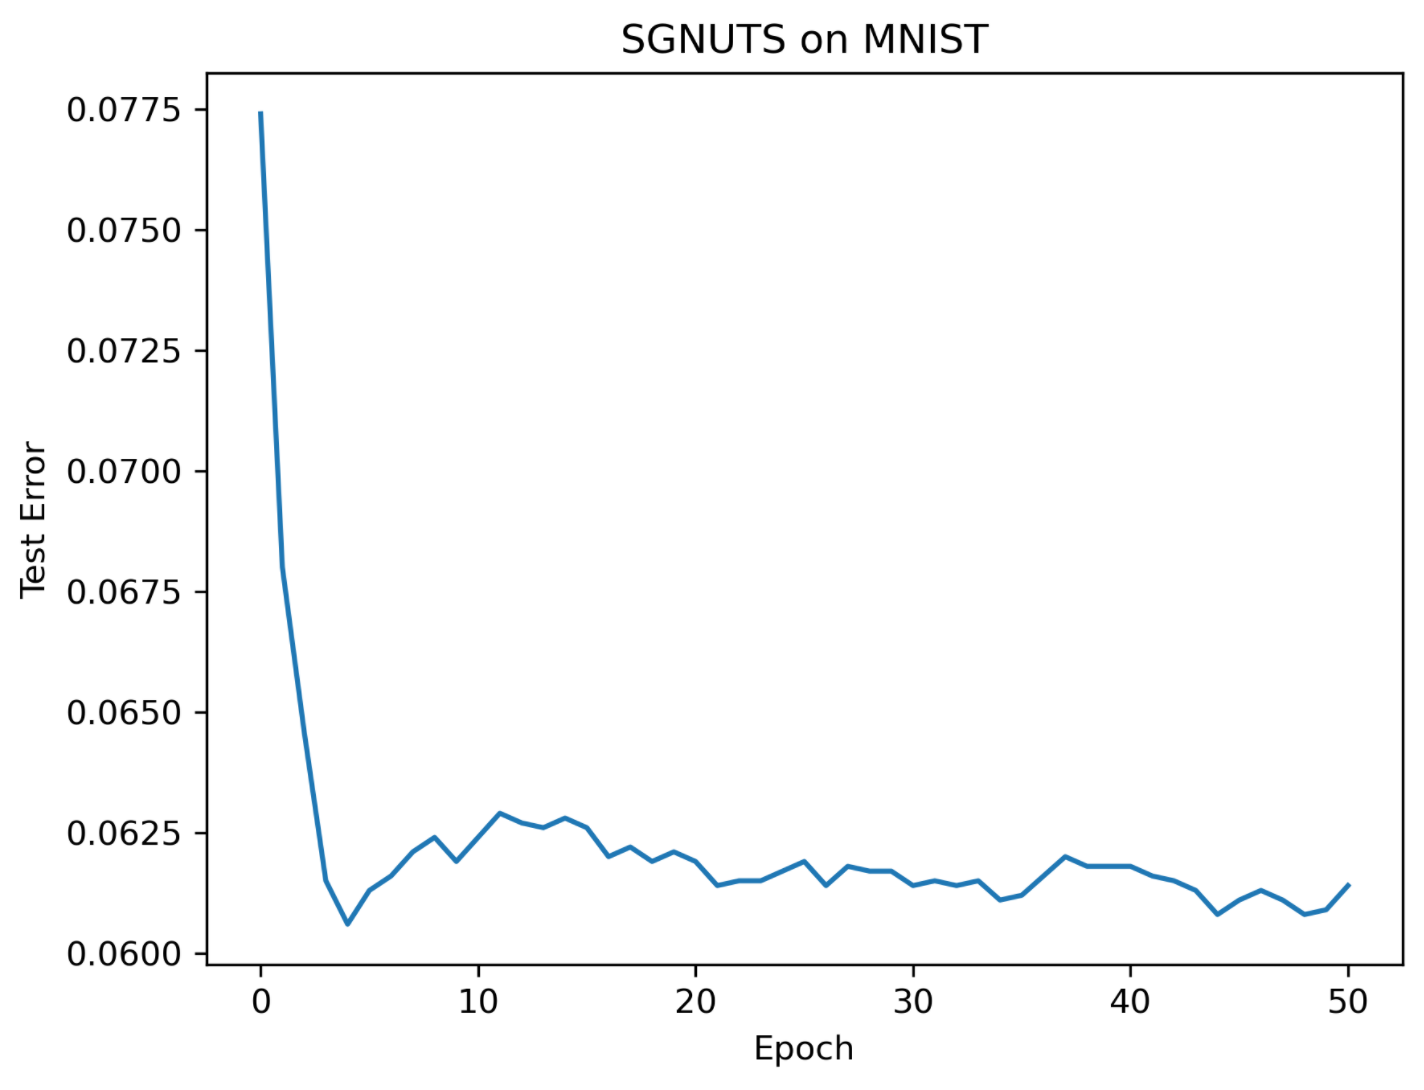
\includegraphics[width=70mm]{parts/Images/SGNUTS_MNIST.png}
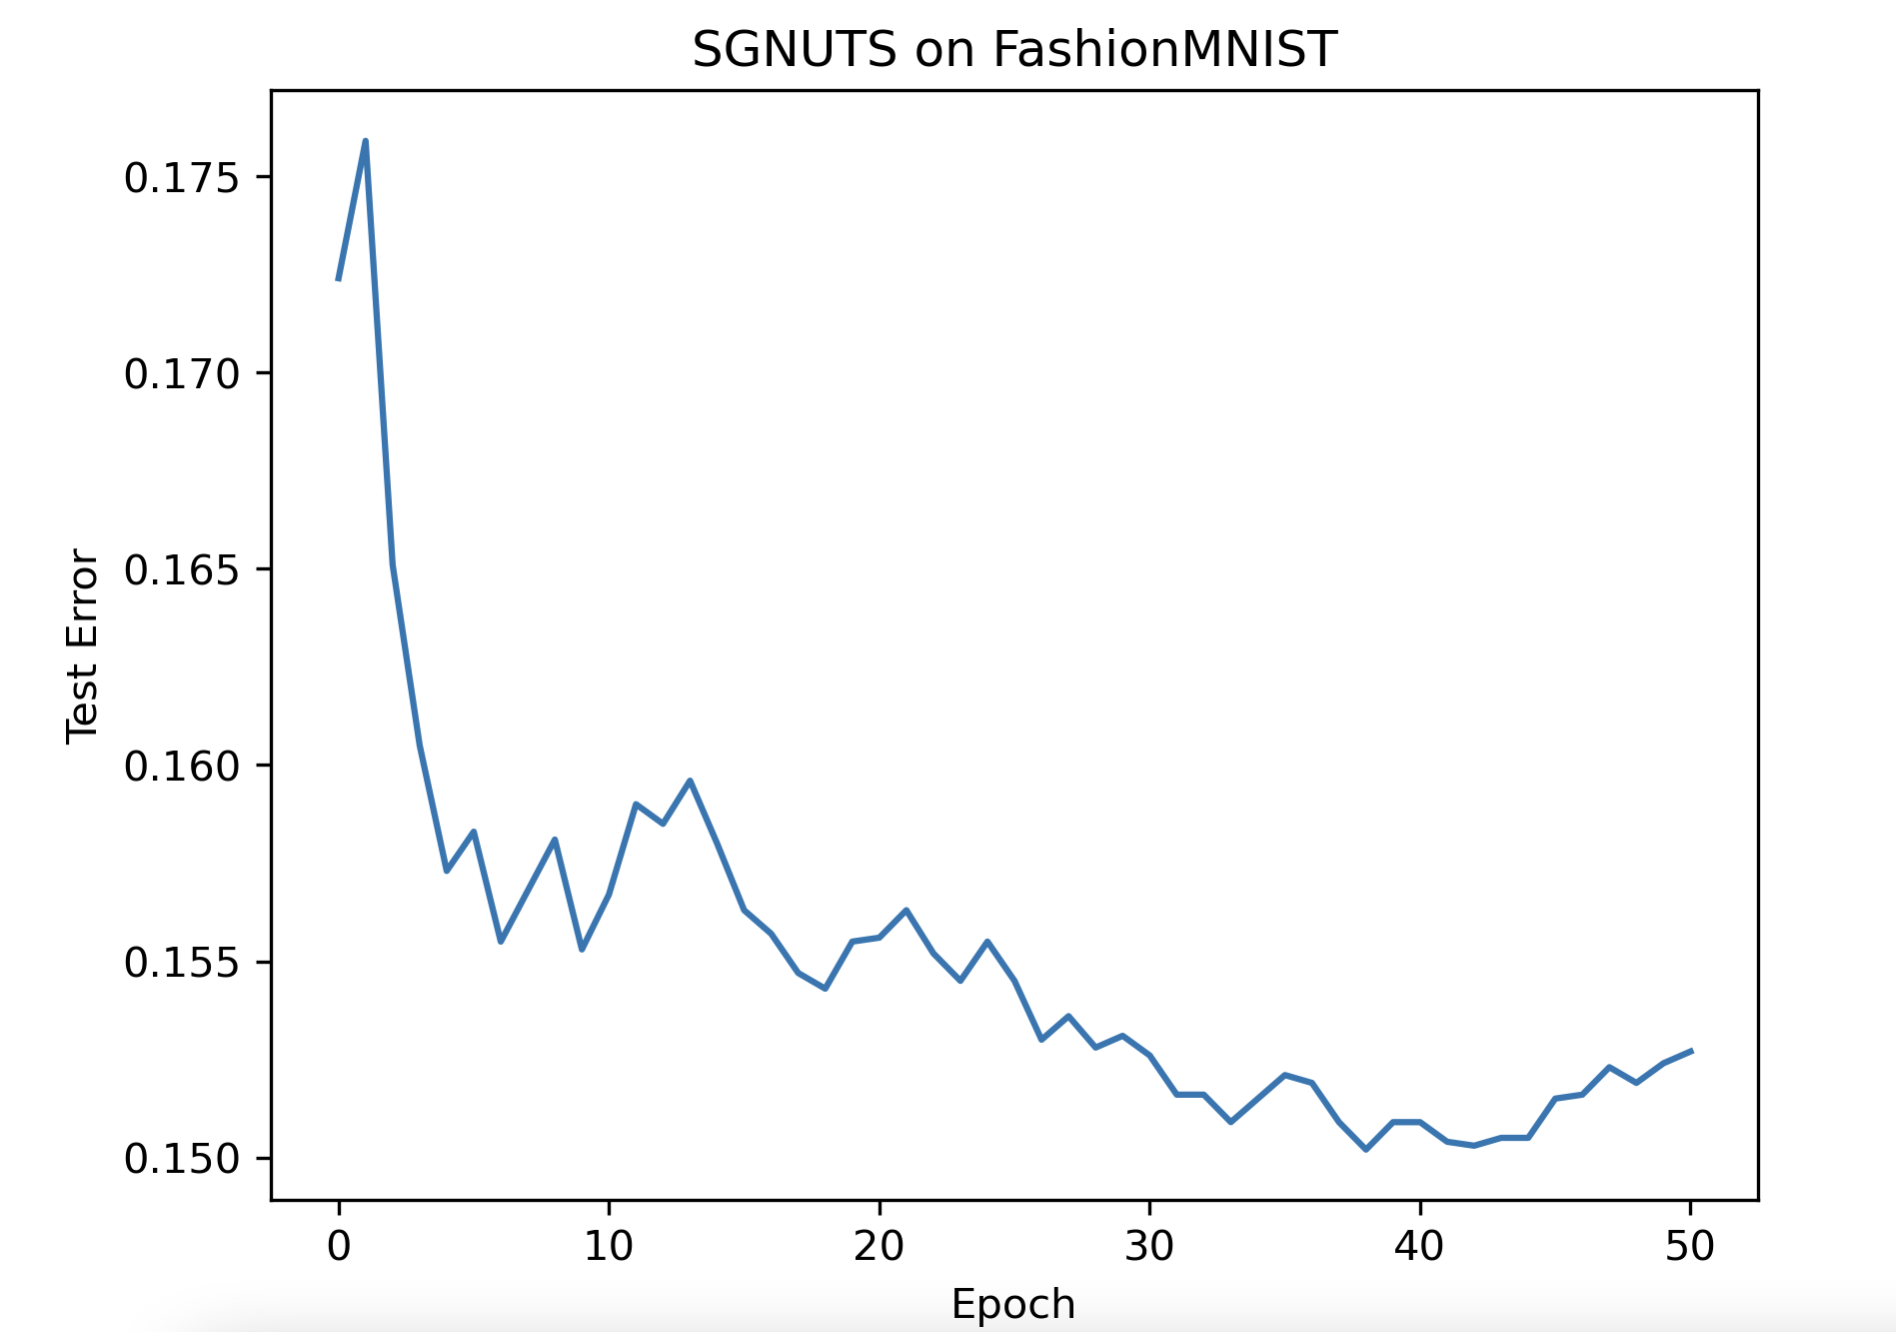
\includegraphics[width=75mm]{parts/Images/SGNUTS_Fashion.png}
\caption{Classifying MNIST and FashionMNIST with SGNUTS}
\label{SGNUTS_results}
\end{figure}

The final accuracies were 0.94 for MNIST and 0.85 for FashionMNIST which are similar to the accuracies obtained using SGNUTS (0.97 and 0.86 respectively). This accuracy demonstrates that there is convergence to the true posterior in SGNUTS. This suggests that, like SGHMC itself, the SGNUTS Markov Chain is likely reversible in some (non traditional) sense. Denoting the posterior as $\pi(\theta, r)$, and transition kernels as $P(\theta, r| \theta', r')$, it is shown in (\cite{sghmc}) that SGHMC satisfies
$$ \pi(\theta,r)P_{SGHMC}(\theta,r|\theta',r') = \pi(\theta',-r')P_{SGHMC}(\theta',-r'|\theta,-r)$$

and it is suggested that this is the reason why the SGHMC algorithm works, despite not being reversible in the traditional sense. It would be interesting to consider if a similar property holds for $P_{SGNUTS}$.

While accurate, SGNUTS is slower to run than SGHMC to produce a single sample. It does however reach relatively high accuracies in a short amount of time. We measured the accuracy after the first epoch of SGHMC and NUTS as we changed the number of warmup epochs, and we measured how long they took to train.

\begin{center}
\begin{tabular}{ccccc} 
\hline
Number of Warmup-Epochs &\multicolumn{2}{c}{SGHMC}& \multicolumn{2}{c}{SGNUTS} \\
& Accuracy & Time (s) & Accuracy & Time (s) \\
 \hline
 0 &0.7747  &  3.2&0.8715&28.3\\ 
 1 & 0.5764 & 4.5 &0.9296&127.2\\ 
 2 & 0.4141 & 6.2&0.9231&453.3\\ 
 5 &0.6471& 11.4 &&\\ 
 10 &0.7100& 20.3 &&\\ 
 25 &0.8866& 50.2 &&\\ 
 \hline
\end{tabular}
\end{center}

In particular, SGNUTS reached an accuracy of 0.87 in 28s, while SGHMC reached 0.89 in 50s. This suggests a new algorithm that uses both SGNUTS and SGHMC - we could run a single epoch of SGNUTS so that we quickly approach the posterior distribution, at which point we switch to running SGHMC. It should be noted the speed up suggested by the above results would only be 30s seconds, however maybe on more complex datasets this could be larger. It would be interesting to investigate this if we had more time.
	%!TEX root = ../report.tex

\section{Conclusion}

For this project, we have implemented a number of algorithms for the purpose of replicating and extending the experiments in \cite{sghmc}. We opted for a close integration with Pyro which allowed us to make use of its probabilistic programming framework. 

Replicating the analysis in \cite{sghmc} we compared the performance of SGHMC with related samplers. We confirmed their results that on the toy models SGHMC samples accurately from the posterior and efficiently samples from correlated distributions. Next, we tested SGHMC on a BNN for classifying MNIST digits, comparing it to SGLD, SGD and SGD with momentum. We obtained similar results to the original experiment. Moreover, we expanded the analysis by testing SGMHC on a BNN for the Fashion-MNIST dataset and a CNN for CIFAR10. In both cases SGMHC performed very well. In the former we further compared SGLD, SGD and SGD with momentum, with SGMHC producing the superior performance. Given the close integration of our codebase with Pyro, it is easy to extend to further models and datasets, which we would do if given more time.

As a further extension, we briefly compared SGHMC with the more popular variational inference method, using our BNN on the MNIST dataset. Over a large number of epochs SGHMC performs better than VI. However, the latter converges faster, and requires fewer samples to give a representative picture of the posterior. With more time, we would like to investigate this further, for example by comparing the sampling efficiency more in-depth.

Our implementation of SGHMC provided the option of estimating the noise model using the observed information, as suggested in \cite{sghmc}. Given more time, we would like to investigate alternative methods of estimating the noise model, ideally ones less computationally expensive.

Our last extension to \cite{sghmc} was the specification and implementation of the model method SGNUTS, which combines SGHMC with the No-U-Turn Sampler. In spite of the lack of reversibility of the corresponding Markov process, our algorithm performs well on a BNN for the MNIST and Fashion-MNIST datasets. We found that while SGNUTS takes longer than SGHMC to produce a single sample, but reaches high accuracies in a relatively small number of steps. If we were to continue this project, we would investigate in more detail the theoretical and practical aspects of SGNUTS.

	\printbibliography


\end{document}